\documentclass[]{article}
\usepackage[T1]{fontenc}
\usepackage{lmodern}
\usepackage{amssymb,amsmath}
\usepackage{ifxetex,ifluatex}
\usepackage{fixltx2e} % provides \textsubscript
\usepackage{graphicx}

% Proper A4 geometry:
\usepackage[hmargin=2.5cm,vmargin=2.5cm,paper=a4paper]{geometry}
\usepackage{lastpage} % for the number of the last page in the document

% fancy header
\usepackage{fancyhdr}
\pagestyle{fancy}

% header content
\lhead{
\includegraphics[width=0.15\textwidth]{./img/dikw-logo.png}}
\chead{Speedtest Analysis of 4G Mobile Networks}
\rhead{}

% footer
\renewcommand{\footrulewidth}{0.5pt}
%\lfoot{left footer content}
\cfoot{\tiny The analysis was performed by DIKW Consulting on behalf of T-Mobile, based on Ookla's NetMetrics Data from Speedtest.net \newline
\normalsize Page \thepage\ of \pageref{LastPage}}
%\rfoot{right footer content}

% use upquote if available, for straight quotes in verbatim environments
\IfFileExists{upquote.sty}{\usepackage{upquote}}{}
\ifnum 0\ifxetex 1\fi\ifluatex 1\fi=0 % if pdftex
  \usepackage[utf8]{inputenc}
\else % if luatex or xelatex
  \ifxetex
    \usepackage{mathspec}
    \usepackage{xltxtra,xunicode}
  \else
    \usepackage{fontspec}
  \fi
  \defaultfontfeatures{Mapping=tex-text,Scale=MatchLowercase}
  \newcommand{\euro}{€}
\fi

% use microtype if available
\IfFileExists{microtype.sty}{\usepackage{microtype}}{}
\usepackage{color}
\usepackage{fancyvrb}
\newcommand{\VerbBar}{|}
\newcommand{\VERB}{\Verb[commandchars=\\\{\}]}
\DefineVerbatimEnvironment{Highlighting}{Verbatim}{commandchars=\\\{\}}
% Add ',fontsize=\small' for more characters per line
\usepackage{framed}
\definecolor{shadecolor}{RGB}{248,248,248}
\newenvironment{Shaded}{\begin{snugshade}}{\end{snugshade}}
\newcommand{\KeywordTok}[1]{\textcolor[rgb]{0.13,0.29,0.53}{\textbf{{#1}}}}
\newcommand{\DataTypeTok}[1]{\textcolor[rgb]{0.13,0.29,0.53}{{#1}}}
\newcommand{\DecValTok}[1]{\textcolor[rgb]{0.00,0.00,0.81}{{#1}}}
\newcommand{\BaseNTok}[1]{\textcolor[rgb]{0.00,0.00,0.81}{{#1}}}
\newcommand{\FloatTok}[1]{\textcolor[rgb]{0.00,0.00,0.81}{{#1}}}
\newcommand{\CharTok}[1]{\textcolor[rgb]{0.31,0.60,0.02}{{#1}}}
\newcommand{\StringTok}[1]{\textcolor[rgb]{0.31,0.60,0.02}{{#1}}}
\newcommand{\CommentTok}[1]{\textcolor[rgb]{0.56,0.35,0.01}{\textit{{#1}}}}
\newcommand{\OtherTok}[1]{\textcolor[rgb]{0.56,0.35,0.01}{{#1}}}
\newcommand{\AlertTok}[1]{\textcolor[rgb]{0.94,0.16,0.16}{{#1}}}
\newcommand{\FunctionTok}[1]{\textcolor[rgb]{0.00,0.00,0.00}{{#1}}}
\newcommand{\RegionMarkerTok}[1]{{#1}}
\newcommand{\ErrorTok}[1]{\textbf{{#1}}}
\newcommand{\NormalTok}[1]{{#1}}
\usepackage{longtable,booktabs}

\usepackage{graphicx}
% Redefine \includegraphics so that, unless explicit options are
% given, the image width will not exceed the width of the page.
% Images get their normal width if they fit onto the page, but
% are scaled down if they would overflow the margins.
\makeatletter
\def\ScaleIfNeeded{%
  \ifdim\Gin@nat@width>\linewidth
    \linewidth
  \else
    \Gin@nat@width
  \fi
}
\makeatother
\let\Oldincludegraphics\includegraphics
{%
 \catcode`\@=11\relax%
 \gdef\includegraphics{\@ifnextchar[{\Oldincludegraphics}{\Oldincludegraphics[width=\ScaleIfNeeded]}}%
}%

\ifxetex
  \usepackage[setpagesize=false, % page size defined by xetex
              unicode=false, % unicode breaks when used with xetex
              xetex]{hyperref}
\else
  \usepackage[unicode=true]{hyperref}
\fi
\hypersetup{breaklinks=true,
            bookmarks=true,
            pdfauthor={Hugo Koopmans},
            pdftitle={Independent Speed test Analysis of 4G Mobile Networks Performed by DIKW Consulting},
            colorlinks=true,
            citecolor=blue,
            urlcolor=blue,
            linkcolor=magenta,
            pdfborder={0 0 0}}
\urlstyle{same}  % don't use monospace font for urls
\setlength{\parindent}{0pt}
\setlength{\parskip}{6pt plus 2pt minus 1pt}
\setlength{\emergencystretch}{3em}  % prevent overfull lines
\setcounter{secnumdepth}{5}

%
\includegraphics[width=0.15\textwidth]{./img/dikw-logo.png} ~\\[1cm]
\title{Independent Speed test Analysis of 4G Mobile Networks Performed by DIKW
Consulting}
\author{Hugo Koopmans}
\date{06-07-2015}

% Definition of \maketitle
\makeatletter         
\def\@maketitle{
%\raggedright
\begin{center}

\includegraphics[width = 75mm]{./img/dikw-logo.png} \\[5cm]
{\Large  \@title }\\[4ex] 
{\@author}\\[4ex] 
\@date\\[8ex]
\end{center}}
\makeatother

\begin{document}
\maketitle

\newpage


{
\hypersetup{linkcolor=black}
\setcounter{tocdepth}{2}
\tableofcontents
}

\newpage

\newpage

\subsection{Colophon}\label{colophon}

This analysis is performed by DIKW Consulting.

DIKW Consulting is a consulting firm that takes her customers on the
path from Data to information to Knowledge to Wisdom. Our expertise is
in the field of data logistics, data warehousing, data mining and
machine learning.

T-Mobile has asked DIKW Consulting to perform this test as an
independent third party. DIKW Consulting was paid to perform this test
by T-mobile and has no other intentions then to perform this test by
it's own high quality standards. The analysis was performed by generally
accepted and approved standards and statistical methods using open
source tools.

We let the data speak for itself.

If you have questions you can contact \href{http://www.dikw.nl}{DIKW
Consulting}. If you want to repeat this test by yourself you are welcome
to do so, all necessary scripts are available on GitHub. The data is
commercially available at \href{http://www.ookla.com/}{Ookla}.

This analysis, method, tools and scripts are open sourced and placed on
GitHub, see the read-me on the GitHub
\href{https://github.com/hugokoopmans/ookla-speedtest-analysis}{repository}.

For questions contact Hugo Koopmans at
\href{mailto:hugo.koopmans@dikw.com}{\nolinkurl{hugo.koopmans@dikw.com}}
or +31 6 43106780

\subsection{Code generation}\label{code-generation}

This is an R Markdown document. Markdown is a simple formatting syntax
for authoring HTML, PDF, and MS Word documents. For more details on
using R Markdown see \url{http://rmarkdown.rstudio.com}.

\newpage

\section{Abstract}\label{abstract}

In this document we have conducted a statistical analysis of Ookla's
NetMetrics data from speedtest.net. Ookla provides commercially
available speed test data collected by their mobile app on the three
main mobile platforms, Android, iOS and Windows mobile. We will load all
the raw speed test data into a database, analyse the data ot the top
three operators(T-Mobile, Vodafone and KPN) and perform a test on how
fast their respective 4G networks are. Our test will be on download
speed, upload speed and latency(or ping).

The speed test data that is provided by Ookla's NetMetrics data from
speedtest.net and obtained by T-Mobile is of April, May and June 2015.
We will analyse and validate the data step by step. After investigation
on suspicious testing circumstances, such as, but not limited to,
devices, location, theoretical maximum speeds and specific dates the
data is ready to be subjected to a significance test. This test will be
done for all the data in the coverage area and for the biggest twenty
cities in the Netherlands.

The result of these tests will give an answer to whether or not T-Mobile
has on average a faster 4G network than Vodafone and/or KPN, based on
the three metrics upload speed, download speed and latency.

\newpage

\section{Introduction}\label{introduction}

This document is a report of a statistical analysis of 4G network speed
test data. The time period we consider is Q2 2015 so the months April,
May and June of 2015 are in scope. We perform an analysis of
\href{http://www.ookla.com/}{Ookla} NetMetrics Data data on three
different measures:

\begin{itemize}
\itemsep1pt\parskip0pt\parsep0pt
\item
  download speed
\item
  upload speed
\item
  latency(or ping)
\end{itemize}

On these metrics we compare the three major providers of 4G mobile
networks in the Netherlands, Vodafone, KPN and T-Mobile.

This analysis is set up as follows:

\begin{itemize}
\itemsep1pt\parskip0pt\parsep0pt
\item
  Step 1: Data Collection
\item
  Step 2: Data preprocessing\\
\item
  Step 3: Data analysis
\item
  Step 4: Test design
\item
  Step 5: Test results coverage area
\end{itemize}

In section 8 we provide the conclusion, and additionally the analysis
and results of the Top 20 cities per city is presented in section 9.

\section{Step 1 : Data Collection}\label{step-1-data-collection}

The data was downloaded from Ookla servers by T-Mobile. For this
analysis we use a PostgreSQL database that is locally installed.

The data is loaded from three different files, each file resembling a
mobile platform (Android,iPhone and Windows mobile). The data is loaded
as-is as it was received from the Ookla server. Scripts to load this
data directly into a PostgreSQL database can be found in the GitHub
repository.

All scripts to process the data are in SQL(available on GitHub) or
R(included in this document, thanks to
\href{http://yihui.name/knitr/}{knitr})

Let's get the data and do some basic counts.

\subsection{The raw data}\label{the-raw-data}

We load the raw files, downloaded from the Ookla server, into individual
tables per mobile platform. In the table below we count the number of
speed tests per mobile platform in Q2/2015.

\begin{longtable}[c]{@{}lr@{}}
\caption{Raw test data counts}\tabularnewline
\toprule
& Counts\tabularnewline
\midrule
\endfirsthead
\toprule
& Counts\tabularnewline
\midrule
\endhead
Android & 179406\tabularnewline
iOS & 109980\tabularnewline
Windows & 7438\tabularnewline
Sum & 296824\tabularnewline
\bottomrule
\end{longtable}

\newpage
So we start this analysis with in total 296824 speed tests, which are
represented as rows in the data set commercially downloaded from Ookla.

\subsection{Speedtest.net data}\label{speedtest.net-data}

Ookla designed their speed test in such a way that the results are as
robust as possible. Ookla's speedtest.net is the de-facto standard for
internet speed testing. According to
\url{http://www.ookla.com/netmetrics}, NetMetrics is the choice of
nearly every Fortune 500 ISP and Mobile Provider in the world. For more
information please visit
\href{https://support.speedtest.net/hc/en-us}{Speeedtest.net}.

\subsection{Sample test data from
Ookla}\label{sample-test-data-from-ookla}

Ookla has some random sample data available, this data can be used to
validate our method. To validate the test result one would need the
specific data of the Netherlands.

A sample set of Ookla NetMetrics data can be found
\href{http://www.ookla.com/netmetrics}{here}. The files differ per
mobile platform. The file descriptors for all three mobile platforms are
listed below.

\subsubsection{Android header
descriptives}\label{android-header-descriptives}

\footnotesize

\begin{verbatim}
test_id - unique id of test in our system
device_id - unique device id in our system
android_fingerprint
test_date - YYYY-MM-DD HH:MM:SS in Pacific time (we can accommodate different time zones if needed)
client_ip - ip of client
download_kbps - download speed in kilobits per second
upload_kbps - upload speed in kilobits per second
latency_ms - ping in milliseconds
server_name - name of server tested to (name of city it is located in)
server_country - country name of server
server_country_code - country code of server
server_latitude - latitude of server tested to
server_longitude - longitude of server tested to
server_sponsor_name - sponsor name of server
client_country - country name of the client
client_country_code - country code of the client
client_region - region name of client (this will be state in the US)
client_region_code - region code of client
client_city - city of client
client_latitude - latitude of client (GPS or Maxmind when location services disabled)
client_longitude - longitude of client (GPS or Maxmind when location services disabled)
miles_between - miles between the client and the server tested to
connection_type - http://developer.android.com/reference/android/telephony/TelephonyManager.html
   0=unknown,1= Cell, 2=Wifi, 3=Gprs, 4=Edge, 5=Utms, 6=Cdma, 7=Evdo0, 8=EvdoA, 9=OnexRTT, 
   10=Hsdpa, 11=Hspa, 12=Iden, 13=Ehrpd, 14=EvdoB, 15=Lte, 16=Hsupa, 17=Hspap
isp_name  - name of ISP (Maxmind)
is_isp    - 0=Corporation/Academic, 1=ISP
network_operator_name - Mobile Carrier Name http://developer.android.com/reference/android
   /telephony/TelephonyManager.html#getNetworkOperatorName()
network_operator_code - MCC + MNC  http://developer.android.com/reference/android
   /telephony/TelephonyManager.html#getNetworkOperator() 
brand - http://developer.android.com/reference/android/os/Build.html#BRAND 
device - http://developer.android.com/reference/android/os/Build.html#DEVICE 
hardware - http://developer.android.com/reference/android/os/Build.html#HARDWARE 
build_id - http://developer.android.com/reference/android/os/Build.html#ID 
manufacturer - http://developer.android.com/reference/android/os/Build.html#MANUFACTURER 
model - http://developer.android.com/reference/android/os/Build.html#MODEL 
product - http://developer.android.com/reference/android/os/Build.html#PRODUCT  
cdma_cell_id - http://developer.android.com/reference/android/telephony/cdma/package-summary.html 
gsm_cell_id - http://developer.android.com/reference/android/telephony/gsm/package-summary.html 
location_type - 0 = unknown, 1 = GPS, 2 = GeoIP
sim_network_operator_name - Mobile Carrier Name from the SIM
sim_network_operator_code - MCC + MNC from the SIM  http://en.wikipedia.org/wiki/Mobile_Country_Code 
\end{verbatim}

\normalsize

\subsubsection{iOS header descriptives}\label{ios-header-descriptives}

\footnotesize

\begin{verbatim}
test_id - unique id of test in our system
device_id - unique device id in our system
test_date - YYYY-MM-DD HH:MM:SS in Pacific time (we can accommodate different time zones if needed)
client_ip - ip of client 
download_kbps - download speed in kilobits per second
upload_kbps - upload speed in kilobits per second
latency_ms - ping in milliseconds
server_name - name of server tested to (name of city it is located in)
server_country - country name of server
server_country_code - country code of server
server_latitude - latitude of server tested to
server_longitude - longitude of server tested to
server_sponsor_name - sponsor name of server
client_country - country name of the client
client_country_code - country code of the client
client_region - region name of client (this will be state in the US)
client_region_code - region code of client
client_city - city of client
client_latitude - latitude of client (GPS or Maxmind when location services disabled)
client_longitude - longitude of client (GPS or Maxmind when location services disabled)
miles_between - miles between the client and the server tested to
connection_type - 0=unknown, 1=cell, 2=wifi, 3=GPRS, 4=Edge, 5=WCDMA, 6=HSDPA, 
   7=HSUPA, 8=CDMA1x, 9=CDMAEVDORev0, 10=CDMAEVDORevB, 11=eHRPD, 12=LTE 
isp_name  - name of ISP (Maxmind) 
is_isp    - 0=Corporation/Academic, 1=ISP
carrier_name - http://developer.apple.com/library/ios/documentation/NetworkingInternet
   /Reference/CTCarrier/Reference/Reference.html#//apple_ref/occ/instp/CTCarrier/carrierName 
iso_country_code - http://developer.apple.com/library/ios/documentation/NetworkingInternet
   /Reference/CTCarrier/Reference/Reference.html#//apple_ref/occ/instp/CTCarrier/isoCountryCode 
mobile_country_code - http://developer.apple.com/library/ios/documentation/NetworkingInternet
   /Reference/CTCarrier/Reference/Reference.html#//apple_ref/occ/instp/CTCarrier/mobileCountryCode 
mobile_network_code - http://developer.apple.com/library/ios/documentation/NetworkingInternet
   /Reference/CTCarrier/Reference/Reference.html#//apple_ref/occ/instp/CTCarrier/mobileNetworkCode
model - iPad, iPhone, iPod Touch 
version - iOS version
location_type - 0 = unknown, 1 = GPS, 2 = GeoIP
\end{verbatim}

\normalsize

\subsubsection{Windows Mobile header
descriptives}\label{windows-mobile-header-descriptives}

\footnotesize

\begin{verbatim}
test_id - unique id of test in our system
device_id - unique device id in our system
test_date - YYYY-MM-DD HH:MM:SS in Pacific time (we can accommodate different timezones if needed)
client_ip - ip of client 
download_kbps - download speed in kilobits per second
upload_kbps - upload speed in kilobits per second
latency_ms - ping in milliseconds
server_name - name of server tested to (name of city it is located in)
server_country - country name of server
server_country_code - country code of server
server_latitude - latitude of server tested to
server_longitude - longitude of server tested to
server_sponsor_name - sponsor name of server
client_country - country name of the client
client_country_code - country code of the client
client_region - region name of client (this will be state in the US)
client_region_code - region code of client
client_city - city of client
client_latitude - latitude of client (GPS or Maxmind when location services disabled)
client_longitude - longitude of client (GPS or Maxmind when location services disabled)
miles_between - miles between the client and the server tested to
connection_type - 0=unknown, 1=cell, 2=wifi, 3=GPRS, 4=1XRTT, 5=EVDO, 6=EDGE, 7=3G, 
   8=HSPA, 9=EVDV, 10=PassThru, 11=LTE, 12=EHRPD
isp_name  - name of ISP (Maxmind) 
is_isp    - 0=Corporation/Academic, 1=ISP
carrier_name - AT&T, Verizon etc 
manufacturer - Nokia, HTC, etc.
device_name - name of the device for e.g. "HD7 T9292" 
hardware_version - device hardware version e.g. "1.0.0.0"
firmware_version - device firmware_version e.g. "1232.2107.1241.1001"
location_type - 0 = unknown, 1 = GPS, 2 = GeoIP
\end{verbatim}

\normalsize

\section{Step 2: Data preprocessing}\label{step-2-data-preprocessing}

In order to compare the data from the three different mobile platforms,
we need to perform basic data transformations and merge it into one
table.

Following that, in this preprocessing and analysis step we validate the
data on the following points: 1. Are there any specific individual
devices that perform a suspiciously high number of tests? 2. We apply
filters so only the tests from the three operators we are interested in
remain. 3. We apply filters so only tests done on 4G technology remain.
4. We are only interested in the coverage area in which all three
operators claim to have 4G coverage. 5. We look at speed test results
that are ``too good to be true'' that is, measured speeds that are above
the theoretical maximum possible for that specific technology. We remove
these speed tests. 6. We look at specific coordinates that are very
frequent, depending on the explanation as for why these coordinates are
used to often we remove or delete the speed tests per coordinate. 7. We
look at specific dates that have a high number of speed tests for that
day.

After all these checks we end up with a data set that is cleaned and
ready to perform a statistical significance test on the investigated
metrics.

\subsection{Basic data
transformations}\label{basic-data-transformations}

As explained in section 3.3., the data from the three different mobile
platforms comes in different formats and some basic data transformations
are necessary before we can merge it into one table.

First of all, the names for the individual operators are spelled in
various ways (e.g. `T-Mobile NL`, `T-Mobile NL'). Next, we need to map
connection types to the specific technology used (2G, 3G or 4G)
depending on the operating system of the device. For more details on
these transformations, please see the SQL script on GitHub.

After these transformations are performed, we proceed with the checks
and cleaning steps explained at in the previous section.

\subsection{Suspicious devices}\label{suspicious-devices}

Are there any devices that perform tests very frequently?

In order to investigate this, let's look at a frequency plot of devices
that occur at least \textbf{ten} times in each month. On the right hand
side we see devices that are used for testing very often, some of them
even on an hourly basis. Obviously those devices are not in the hands of
real customers so these will be removed from the data set.

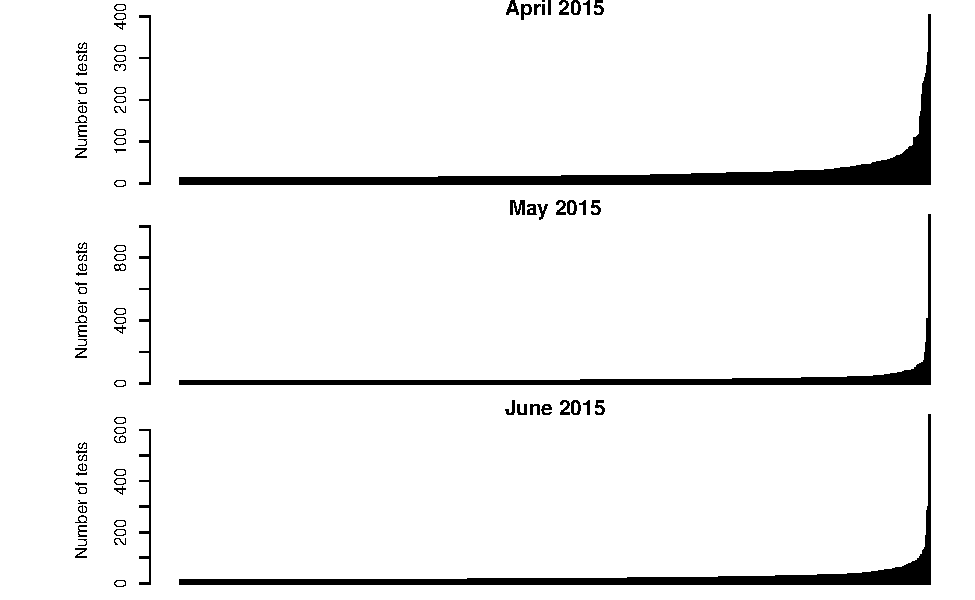
\includegraphics{speedtest-analysis_files/figure-latex/freq-plot-devices-1.pdf}

Based on these plots and the amount of data consumed when performing a
speedtest, we decide to remove specific devices that test more than 30
times a month. These devices are probably used by telecom professionals
for testing purposes. The amount of data consumed per speedtest depends
on the speed: the higher the speed, the more data is consumed. A test on
4G at very high speed can cost up to 100 MBytes per test out of the data
bundle. So, 30 or more tests per month at high speed are equivalent to
approximately 3GB of data usage just spend on tests alone and that is
suspicious. The number 30 by itself is subjective, we could use 25 or 40
depending on what exact number of tests per device you would call
suspicious.

Actually including these are not influencing the results significantly,
but we want to use real customer data as much as possible, not affected
by professionals testing their own (or others) network.

We identify 122 devices in April, 140 devices in May and 133 devices in
June, which in total represent 23456 speed tests. After filtering these
devices the data set has 296824-23456=273368 speed test cases.

\subsection{Top three operators}\label{top-three-operators}

For this analysis we are only interested in the top three operators in
the Netherlands. In the data set, at this point, there are 861 different
operators identified. As we can see in the table below, in which we
ranked the ten most used operators, most of the speed tests were
performed by people using one of the three operators we are interested
in. There are 6534 tests with no identifiable operator. We will filter
out all but the top 3 operators and proceed with speed tests from these
top three operators.

\begin{longtable}[c]{@{}lr@{}}
\caption{Most frequent operators}\tabularnewline
\toprule
Operator & Number of speedtests\tabularnewline
\midrule
\endfirsthead
\toprule
Operator & Number of speedtests\tabularnewline
\midrule
\endhead
KPN NL & 83767\tabularnewline
T-Mobile NL & 57738\tabularnewline
Vodafone NL & 54468\tabularnewline
& 6534\tabularnewline
Carrier & 5481\tabularnewline
Tele2 NL & 5369\tabularnewline
TURKCELL & 5005\tabularnewline
DiGi & 3923\tabularnewline
Telfort NL & 2667\tabularnewline
TIGO & 2500\tabularnewline
\bottomrule
\end{longtable}

The top three operators together are good for 195973 tests conducted all
over the Netherlands in the test period of Q2 2015. We keep only speed
tests from the top three operators.

This leaves 273368 - 77395 = 195973 rows in the data set.

\subsection{Focus on 4G technology}\label{focus-on-4g-technology}

In the raw Ookla Netmetrics data the variable called `connection\_type'
identifies which technology is used, this variable can be transformed
into the network technology used while performing the test.

The variable Connection type defines 4G as connection type 15 for
Android. For iOS connection type 12 is LTE, and for Windows Mobile
connection type 11 is LTE.

Definition of 4G for Android OS from the SQL script(available on GitHub)
:

\begin{Shaded}
\begin{Highlighting}[]
  \KeywordTok{Case}  \KeywordTok{WHEN}  \NormalTok{CONNECTION_TYPE=}\DecValTok{0}         \KeywordTok{THEN} \StringTok{'UNKNOWN'}
    \KeywordTok{WHEN}    \NormalTok{CONNECTION_TYPE }\KeywordTok{in} \NormalTok{(}\DecValTok{1}\NormalTok{,}\DecValTok{2}\NormalTok{)        }\KeywordTok{THEN} \StringTok{'WIFI/CELL'}
    \KeywordTok{WHEN}    \NormalTok{CONNECTION_TYPE }\KeywordTok{in} \NormalTok{(}\DecValTok{3}\NormalTok{,}\DecValTok{4}\NormalTok{)        }\KeywordTok{THEN} \StringTok{'2G'}
    \KeywordTok{WHEN}    \NormalTok{CONNECTION_TYPE=}\DecValTok{15}          \KeywordTok{THEN} \StringTok{'4G'}
    \KeywordTok{WHEN}    \NormalTok{CONNECTION_TYPE }\KeywordTok{between} \DecValTok{5} \KeywordTok{and} \DecValTok{17}    \KeywordTok{THEN} \StringTok{'3G'}
    \KeywordTok{ELSE}    \StringTok{'UNKNOWN'}
  \KeywordTok{END} \KeywordTok{AS} \NormalTok{TECHNOLOGY}
\end{Highlighting}
\end{Shaded}

Below we give an overview of the network technology types available in
the data set.

\begin{longtable}[c]{@{}lrr@{}}
\caption{Technology used in tests}\tabularnewline
\toprule
& Number of cases & Percentage\tabularnewline
\midrule
\endfirsthead
\toprule
& Number of cases & Percentage\tabularnewline
\midrule
\endhead
2G & 2240 & 1.14\tabularnewline
3G & 44394 & 22.65\tabularnewline
4G & 148824 & 75.94\tabularnewline
UNKNOWN & 183 & 0.09\tabularnewline
WIFI/CELL & 332 & 0.17\tabularnewline
\bottomrule
\end{longtable}

\textbf{In the remainder of this analysis we will focus on 4G
technology.}

Filtering on 4G technology leaves 148824 test cases in the data set.

\subsection{Operating systems}\label{operating-systems}

For the top three operators we can look at the type of operating system
used on these devices:

\begin{longtable}[c]{@{}lrrr@{}}
\toprule
& KPN NL & T-Mobile NL & Vodafone NL\tabularnewline
\midrule
\endhead
Android & 42130 & 27157 & 25704\tabularnewline
iOS & 39185 & 29422 & 27175\tabularnewline
Windows & 2452 & 1159 & 1589\tabularnewline
\bottomrule
\end{longtable}

Most of the tests were conducted on iOS closely followed by Android OS.
Windows Mobile devices have limited representation in the data set. In
this test we are not interested in testing the difference in performance
per device or operating system.

\subsection{Geographical coverage area for
4G}\label{geographical-coverage-area-for-4g}

For this test to be fair to all three operators, we limit the comparison
of the test to areas in which all three operators (KPN, Vodafone and
T-Mobile) claim to have 4G coverage at the time of the measurements.
While KPN and Vodafone already claim national 4G coverage, T-Mobile is
still in the process of expanding their 4G network. Therefore, T-Mobile
4G coverage area is extended every month. This means that some areas
only got 4G coverage during Q2 2015, the period of the test. All of the
top 20 cities in the Netherlands, which we will analyze per city, had 4G
enabled prior to Q2 2015.

\subsubsection{Coordinates with very high number of
tests}\label{coordinates-with-very-high-number-of-tests}

Are there any locations, or coordinates, that occur very often in the
investigated 4G area? If we join the coordinates latitude and longitude
together and look at the most frequent occurrences we see that there are
indeed some coordinates that are very frequent. How do these exact same
coordinates end up in the data? To understand this we need to explain a
bit more on how the Ookla Speed test application gets the coordinates
from a mobile
device(\href{https://support.speedtest.net/hc/en-us/articles/203845480-Mobile-Test-Server-Selection}{read
more online}). There are several scenario's that can be the case: 1)The
customer has approved the application access to the GPS coordinates of
his/her device. 2)For some reason the app cannot read the GPS
coordinates from the device at the time of the test. This reason can be
of different origins, the user has blocked access or we are in a
building or there are other technical reasons why the exact GPS
coordinates cannot be accessed.

Whenever the exact coordinates are not available, due to measurement
issues or because the customer is not allowing the application to use
the GPS coordinates Ookla uses GEO-IP. GEO-IP is a online service to
estimate the physical location of an ip-internet address (more online
\href{https://www.maxmind.com/en/geoip2-services-and-databases}{from
maxmind} ).

\begin{longtable}[c]{@{}lr@{}}
\toprule
Coordinates & Count\tabularnewline
\midrule
\endhead
52.3667 , 4.9 & 37777\tabularnewline
52.35 , 4.9167 & 2235\tabularnewline
52.3666 , 4.9027 & 547\tabularnewline
51.9167 , 4.5 & 453\tabularnewline
52.0938 , 5.1191 & 165\tabularnewline
52.0833 , 4.3 & 162\tabularnewline
51.8833 , 4.5333 & 129\tabularnewline
52.0537 , 4.4924 & 73\tabularnewline
52.1583 , 4.4931 & 69\tabularnewline
51.8796 , 4.5059 & 67\tabularnewline
52.4385 , 4.8264 & 66\tabularnewline
51.8811 , 4.4569 & 64\tabularnewline
52.3881 , 5.2354 & 59\tabularnewline
51.8425 , 5.8528 & 54\tabularnewline
51.81 , 4.6736 & 53\tabularnewline
\bottomrule
\end{longtable}

We asked for an explanation from Ookla on frequent and rounded
coordinates.

Coordinate (52.3667,4.9) : Response from Ookla: \emph{Results are
definitely coming from GEO-IP Coordinates as you know. 2. In a single
day here, there is 191 results from the same IP block to this location.
3. Correct, this is similar to the `Kansas' issue we discussed last
year.}

Coordinate (52.35-4.9167) is in Amsterdam. Question to Ookla: Can we
still assume the measurements are from Amsterdam? Response Ookla:
\emph{Yes, GeoIP is used here. We can assume you are in Amsterdam but
like any other GeoIP location result, the confidence level isn't as high
as it would be if we were able to get location information directly from
the device, meaning if we were able to obtain GPS instead of GEO-IP.}

Coordinate (52.3666-4.9027) is also in Amsterdam(Waterloo plein).

Coordinate (51.9167-4.5) is in Rotterdam. Again with limited precision,
same response as above from Ookla.

Coordinate (52.0666-4.3209) is in The Hague. All cases are tests with
operator equal to ``T-Mobile NL'' also this location is close to the
T-Mobile office in The Hague. We will exclude these tests as potentially
being from T-Mobile employees.

Also see the
\href{https://en.wikipedia.org/wiki/Decimal_degrees}{precision of the
coordinates} denotes the fact that we are unsure about the exact
location.

\textbf{So what do we do with these suspicious coordinates?} The
``Unknown'' location, which has coordinates (52.3667 , 4.9) and is the
default location from Ookla if the GPS cannot pick up the exact location
during the test, we have 37777 speed tests with this coordinate alone.
We will exclude tests performed at this coordinate from the general
analysis. Nevertheless, we will analyse this set the same way we analyse
individual cities, the result for this set can be found as the last city
labeled ``unknown''.

\textbf{Head office locations} We removed 38 tests from coordinates
``52.0666 , 4.3209'' in The Hague. As they are close to the head-office
of T-Mobile and indeed all tests from this location are done from a
T-Mobile network.

We did the same for locations close to the head offices of KPN and
Vodafone. We removed 33 tests from the co-ordinates ``52.0666 4.3479''
(KPN office) and we removed 14 tests from the coordinates ``52.3767
4.9061''" (Vodafone office Amsterdam).

The other locations (``51.9167-4.5'', ``52.35-4.9167'') have been
explained above and there is no knowledge at this point that leads to
exclusion, so these tests remain in the data set.

After removing tests from the coordinates around the head-offices of the
top three providers as described in the above paragraph, together with
37777 from the coordinates ``52.3667 , 4.9'' the data set contains
148824 - = speed tests at this point.

\subsubsection{Mapping test coordiantes to city
boundaries}\label{mapping-test-coordiantes-to-city-boundaries}

To identify the exact 4G coverage area we will use in this analysis, we
use data from CBS. CBS is the Central Bureau of Statistics in the
Netherlands. They provide
\href{http://www.cbs.nl/nl-NL/menu/themas/dossiers/nederland-regionaal/publicaties/geografische-data/archief/2014/2013-wijk-en-buurtkaart-art.htm}{publicly
available} polygon data on cities in the Netherlands. Based on these
geographical city boundaries we map each latitude, longitude coordinate
onto a city.

From T-Mobile we received a list of cities that, at the time of testing,
have 4G coverage. From the data we can see that per city each provider
has sufficient number of speed tests in the data set for the tests to be
representative.

We use city boundaries to not be influenced by exact locations of
network infrastructure.

Online we can get an up to date overview of network coverage for all
three operators (see \href{http://www.4gdekking.nl/}{here}).

This test is not about coverage but about speed of the 4G network.

T-Mobile has the least 4G coverage of the three operators and per end of
Q2 2015 has actual coverage in the following area:

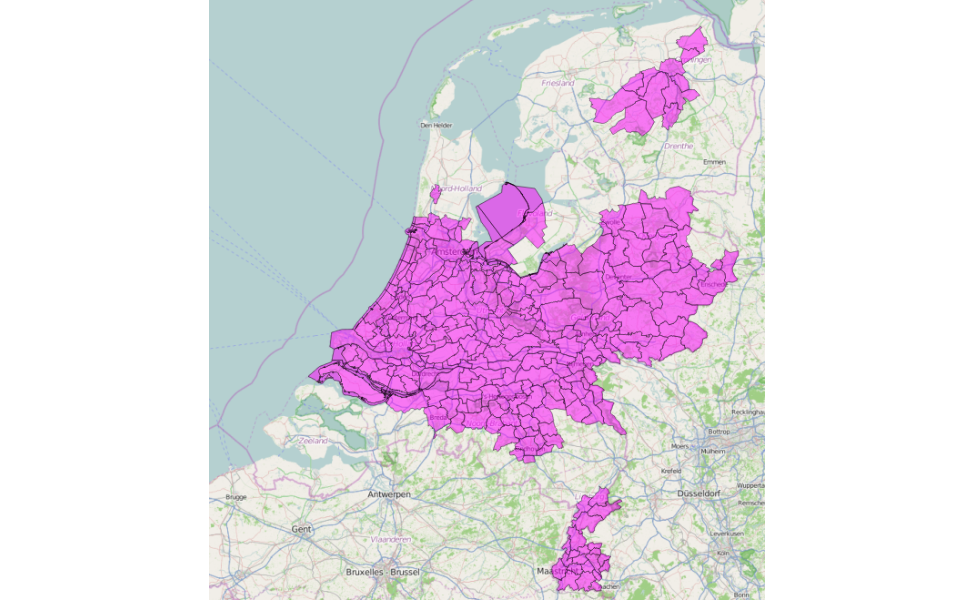
\includegraphics{speedtest-analysis_files/figure-latex/area-1.pdf}

In order to do a fair comparison, we focus only on the area presented in
the picture above.

We do a Geo-spacial filter on the latitude and longitude coordinates
provided in the data set and only keep speed tests that are in any of
the above city boundaries. For the area, defined above, the following
number of tests are available in the data set.

\begin{longtable}[c]{@{}lrr@{}}
\caption{Number of 4G speedtests in the selected coverage
area.}\tabularnewline
\toprule
& Number of tests & percentage\tabularnewline
\midrule
\endfirsthead
\toprule
& Number of tests & percentage\tabularnewline
\midrule
\endhead
KPN NL & 38200 & 39.04\tabularnewline
T-Mobile NL & 33261 & 33.99\tabularnewline
Vodafone NL & 26382 & 26.96\tabularnewline
Sum & 97843 & 100.00\tabularnewline
\bottomrule
\end{longtable}

Areas where T-Mobile announced 4G coverage in Q2 2015:
Helmond,Schijndel,Sint-Oedenrode,Son en Breugel, Uden, Veghel, Laarbeek,
Landerd, Bernheze, Landgraaf, Brunssum, Heerlen, Kerkrade and Schinnen
were added in April ; Leek, Marum, Ooststellingwerf, Opsterland, Assen,
Noordenveld, Brummen, Doesburg, Doetinchem, Duiven, Rheden, Westervoort,
Zevenaar, Lingewaard, Montferland, Beek, Meerssen, Nuth, Stein,
Voerendaal and Valkenburg aan de Geul were added in May; Dalfsen,
Hardenberg, Hellendoorn, Ommen, Raalte, Heerde, Twenterand, Olst-Wijhe,
Onderbanken, Roermond, Maasgouw, Roerdalen, Echt-Susteren,
Sittard-Geleen, Groesbeek, Ubbergen, Boxmeer, Grave, Mill en Sint
Hubert, Bergen (L.), Gennep, Mook en Middelaar, Cuijk, Sint Anthonis,
Haaksbergen, Rijnwaarden, Aalten, Millingen aan de Rijn, Winterswijk,
Oude IJsselstreek, Oost Gelre, Hof van Twente, Berkelland and
Bronckhorst were added in June. All other cities in the TMNL coverage
area had 4G enabled prior to Q2 2015.

Naturally, in the cities where 4G was announced in Q2, almost all of
T-Mobile's 4G speedtests occur after announcing to customers that 4G is
activated, so April, May or June respectively. Even though a very small
number of tests were executed during the extension of the 4G coverage
onto these cities, as 4G sites were being added (so before announcing 4G
coverage in these cities; this is possible as for most 4G capable
phones, the 4G network is selected automatically if available). In the
same cities, KPN and Vodafone speedtests are distributed more evenly
over the entire period of Q2/2015. However, this has no influence on the
test results, as the test results per month do not differ substantially
(please see section 4.6.4).

So we filtered the data set to include only speed tests from the
coverage area, speed tests outside this area are neglected. The data set
now contains - = 97843 speed tests.

\subsubsection{Suspicious speeds}\label{suspicious-speeds}

In the data we check for up and download speeds that are technically
impossible. \emph{Download speeds} for 4G are limited to 150Mbps on the
T-mobile technology.

KPN and Vodafone have a technology called LTE advanced which has a
maximum download speed of 225Mbps.

Any speed tests that had a speed recorded above the technical maximum
for that operator was removed from the data set.

So we remove suspicious measurements in which the \textbf{download}
speed exceeded the maximum theoretical speed per individual operator.

For T-Mobile we removed 4 cases, for Vodafone we removed 1 cases and for
KPN we removed 3 cases, because they where above 150(or 225) MBps.

After removing in total 8 of these suspicious measurements, the data set
contains 97835 speed tests at this point.

Let's do the same for \emph{upload speed}.

The maximum theoretical upload speed is for all operators the same:
maximum upload speed of 50Mbps.

So again we remove suspicious measurements in which the \textbf{upload}
speed exceeded the maximum theoretical speed per individual operator.
For T-Mobile we removed 32 cases, for Vodafone we removed 21 cases and
for KPN we removed 33 cases.

After removing in total 86 of these suspicious measurements the data set
contains 97749 speed tests at this point. \newpage

\subsubsection{Suspicious dates or
times}\label{suspicious-dates-or-times}

We count the number of tests per day for the months April, May and June
of 2015. Again we are looking at any suspicious peaks in the data.

\begin{center}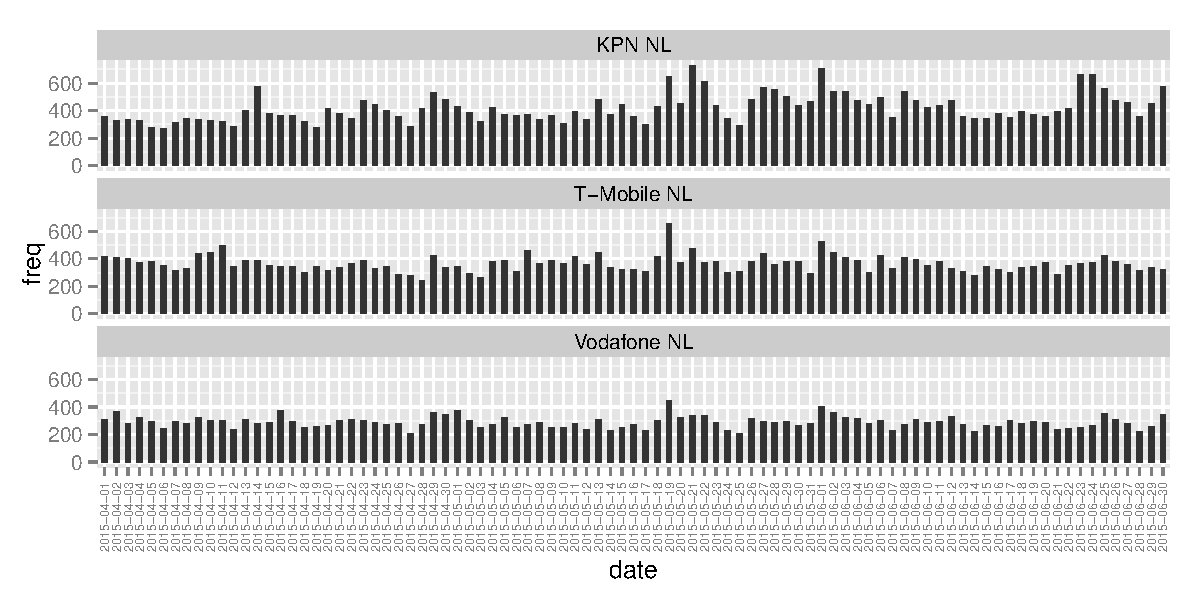
\includegraphics{speedtest-analysis_files/figure-latex/timestamps-1} \end{center}

We find no disturbing or unknown peaks on a specific date.

\begin{longtable}[c]{@{}lrrrr@{}}
\caption{Counts per operator per month}\tabularnewline
\toprule
& 04 april & 05 mei & 06 juni & Sum\tabularnewline
\midrule
\endfirsthead
\toprule
& 04 april & 05 mei & 06 juni & Sum\tabularnewline
\midrule
\endhead
KPN NL & 11056 & 13312 & 13796 & 38164\tabularnewline
T-Mobile NL & 10819 & 11587 & 10819 & 33225\tabularnewline
Vodafone NL & 8832 & 8843 & 8685 & 26360\tabularnewline
Sum & 30707 & 33742 & 33300 & 97749\tabularnewline
\bottomrule
\end{longtable}

Above a count per month per operator in the 4G coverage area. This is
the data set on which we conduct the remainder of the analysis.

In the tables below we list the averages for download speed, upload
speed and latency per operator per month. For KPN we see a large
increase in download and upload speed between April and May, as well as
reduced latency. This is probably a result of KPN adding a substantial
amount of sites in the large cities by activating 4G on the 1800Mhz
frequency. In May 2015, KPN also
\href{http://tweakers.net/nieuws/103231/kpn-biedt-4g+-aan-in-zeven-nederlandse-steden.html}{announced}
LTE-Advanced in the 7 largest cities in The Netherlands. This has an
influence in the increased number of tests, shown in table 7. LTE
advanced can also have a positive influence on average download speed,
because it allows download speeds of up to 225Mbps, provided that the
customer doing the tests has a device that can support this and the
network conditions at the location allow this.

\begin{longtable}[c]{@{}llr@{}}
\caption{Average download speed(Kbps) per operator per
month}\tabularnewline
\toprule
Operator & Month & Average Downloadspeed(Kbps)\tabularnewline
\midrule
\endfirsthead
\toprule
Operator & Month & Average Downloadspeed(Kbps)\tabularnewline
\midrule
\endhead
KPN NL & 04 & 20783.5\tabularnewline
KPN NL & 05 & 29417.4\tabularnewline
KPN NL & 06 & 33042.0\tabularnewline
T-Mobile NL & 04 & 40279.9\tabularnewline
T-Mobile NL & 05 & 39849.7\tabularnewline
T-Mobile NL & 06 & 40659.3\tabularnewline
Vodafone NL & 04 & 28734.2\tabularnewline
Vodafone NL & 05 & 30226.2\tabularnewline
Vodafone NL & 06 & 31379.8\tabularnewline
\bottomrule
\end{longtable}

Table below shows details for upload speed.

\begin{longtable}[c]{@{}llr@{}}
\caption{Average upload speed(Kbps) per operator per
month}\tabularnewline
\toprule
Operator & Month & Average Uploadspeed(Kbps)\tabularnewline
\midrule
\endfirsthead
\toprule
Operator & Month & Average Uploadspeed(Kbps)\tabularnewline
\midrule
\endhead
KPN NL & 04 & 9907.6\tabularnewline
KPN NL & 05 & 13295.7\tabularnewline
KPN NL & 06 & 14439.8\tabularnewline
T-Mobile NL & 04 & 17713.7\tabularnewline
T-Mobile NL & 05 & 17407.0\tabularnewline
T-Mobile NL & 06 & 17210.1\tabularnewline
Vodafone NL & 04 & 13933.4\tabularnewline
Vodafone NL & 05 & 14229.6\tabularnewline
Vodafone NL & 06 & 14273.3\tabularnewline
\bottomrule
\end{longtable}

Table below shows details for latency.

\begin{longtable}[c]{@{}llr@{}}
\caption{Average latency(ms) per operator per month}\tabularnewline
\toprule
Operator & Month & Average Latency(ms)\tabularnewline
\midrule
\endfirsthead
\toprule
Operator & Month & Average Latency(ms)\tabularnewline
\midrule
\endhead
KPN NL & 04 & 43.9\tabularnewline
KPN NL & 05 & 42.5\tabularnewline
KPN NL & 06 & 42.5\tabularnewline
T-Mobile NL & 04 & 37.4\tabularnewline
T-Mobile NL & 05 & 38.6\tabularnewline
T-Mobile NL & 06 & 37.4\tabularnewline
Vodafone NL & 04 & 45.7\tabularnewline
Vodafone NL & 05 & 44.7\tabularnewline
Vodafone NL & 06 & 45.7\tabularnewline
\bottomrule
\end{longtable}

\newpage

\section{Step 3: Data analysis}\label{step-3-data-analysis}

So we have pre-processed the data and looked for anomalies in the data.
If found, we have corrected them. Finally we are ready to compare speed
test data between the three major telecom operators in Netherlands in
the above defined coverage area for the period of Q2 2015.

We will analyse three different metrics:

\begin{itemize}
\itemsep1pt\parskip0pt\parsep0pt
\item
  Download speed
\item
  Upload speed
\item
  Latency
\end{itemize}

There is no useful way to aggregate these individual metrics into one
overall `speed aggregated score'. Most customers are interested in
download speeds, because it affects the most of their experience
(browsing,streaming,downloading etc). Most network speed comparisons
only focus on download speed. However, since upload speed is also
important for posting video's and photos on social media, and ping times
are important for gaming and fast opening of websites these metrics are
also analyzed.

So how are the different metrics distributed?

\subsection{Histogram distributions}\label{histogram-distributions}

A histogram is a graphical representation of the distribution of data.
It is an estimate of the probability distribution of a continuous
variable (quantitative variable),
\href{https://en.wikipedia.org/wiki/Histogram}{more} about histograms on
Wikipedia.

\subsubsection{Download speed}\label{download-speed}

In the histogram below we see download speed in KBps on the horizontal
axis. The number of test cases are plotted as bars, on the vertical axis
we see the count of the number of speed tests in a specific bin (or
range). The histogram gives a visual representation of the distribution
of the data.

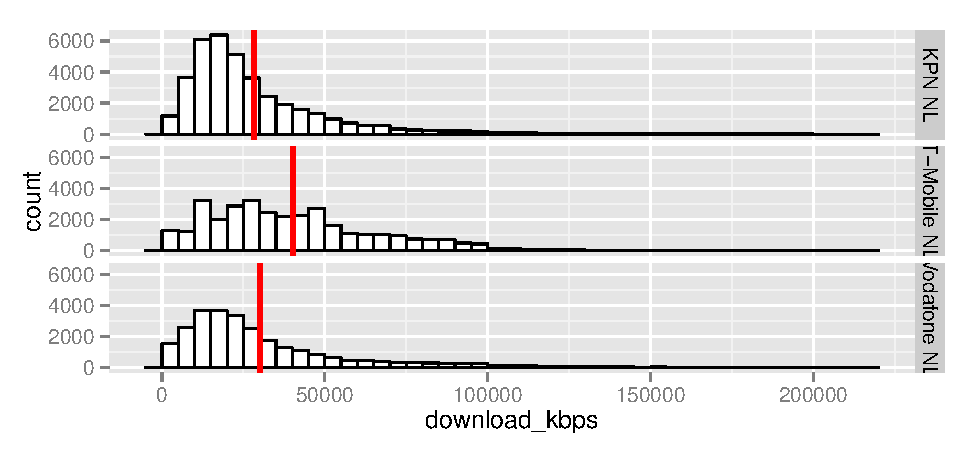
\includegraphics{speedtest-analysis_files/figure-latex/downloadspeed-1.pdf}

We plot the three histograms, one for each operator, right above each
other so the horizontal axes are aligned. The red lines denotes the mean
(or average) speed of all speed tests for the specific operator. If the
red line is placed to the righthandside in this histogram that means the
average speed for this operator is faster. The red line to the left
means the avarage speed is slower. We can see that the red line of
T-Mobile is farthest to the right so T-Mobile apparently has the highest
average download speed.

\subsubsection{Upload speed}\label{upload-speed}

In the histogram below we see upload speed in KBps on the horizontal
axis. The number of test cases are plotted as bars, on the vertical axis
we see the count of the number of speed tests in a specific bin (or
range). The histogram gives a visual representation of the distribution
of the data.

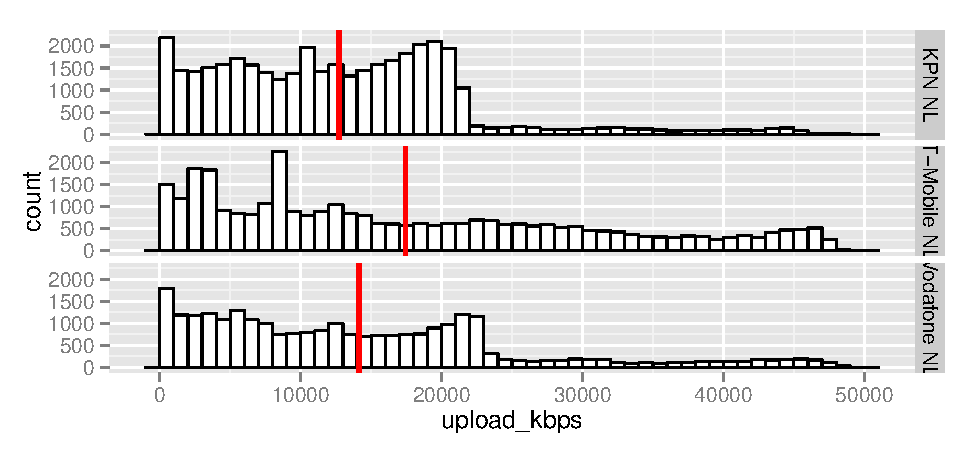
\includegraphics{speedtest-analysis_files/figure-latex/uploadspeed-1.pdf}

We plot the three histograms, one for each operator, right above each
other so the horizontal axes are aligned. The red lines denotes the mean
(or average) speed of all speed tests for the specific operator. If the
red line is placed to the righthandside in this histogram that means the
average speed for this operator is faster. The red line to the left
means the avarage speed is slower. We can see that the red line of
T-Mobile is farthest to the right so T-Mobile apparently has the highest
average upload speed as well.

\subsubsection{Latency}\label{latency}

In the histogram below we see log(latency) speed on the horizontal axis.
The log transformation makes the figure more readable. For the reader,
the horizontal axis shows powers of 10. So 2 actually means \(10^{2}\) =
100 and 5 actually stands for \(10^{5}\) = 10.000 . The number of test
cases are plotted as bars, on the vertical axis we see the count of the
number of speed tests in a specific range. For latency we take the log
so the outlines scale and we can have a look at the shape of the
distribution.

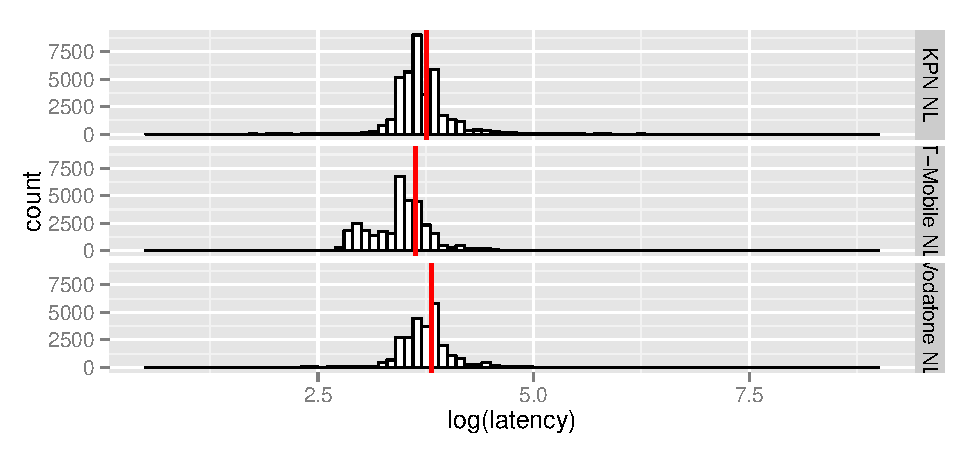
\includegraphics{speedtest-analysis_files/figure-latex/latency-1.pdf}

For latency smaller is better, so in this plot we are looking at which
operator has the smallest latency. Again we see the red lines per
operator. The x axis are on a log scale to these are factors of ten. The
average latency(red line) for T-Mobile is the most to the left, which
means T-Mobile has the smallest average latency of the three operators.

\subsection{Box-plot}\label{box-plot}

In descriptive statistics, a box plot or box-plot is a convenient way of
graphically depicting groups of numerical data through their quartiles.
Box plots may also have lines extending vertically from the boxes
(whiskers) indicating variability outside the upper and lower quartiles,
hence the terms box-and-whisker plot and box-and-whisker diagram.
Outliers may be plotted as individual points.
\href{https://en.wikipedia.org/wiki/Box_plot}{More} about box-plots on
Wikipedia.

\subsubsection{Download speed}\label{download-speed-1}

We see a box plot for each of the operators on the x axis, the vertical
axis shows the speed test values in Kbps. The daimond shape represents
the mean, the thick line represents the median. the black dots on the
top and bottom represent extreme cases. The data is split up into
quartiles, that means four equally sized proportions. The first and
fourth quarter are represented as a line, the second and third as a box.

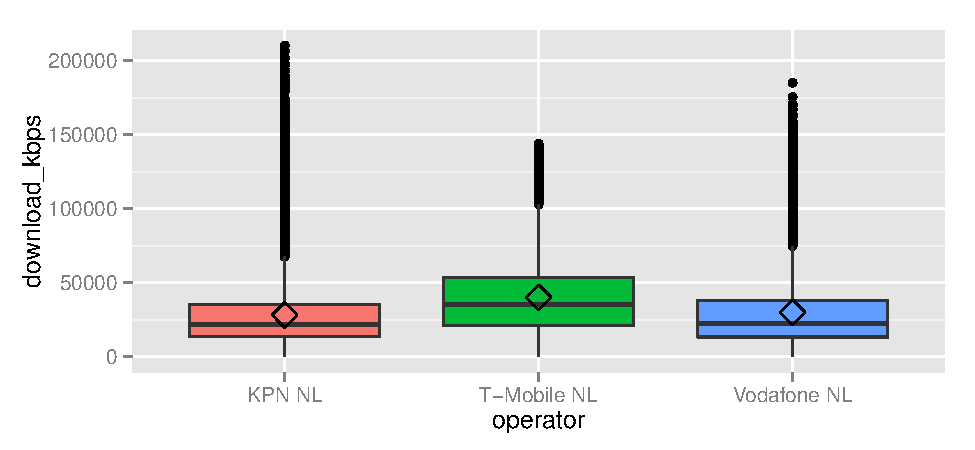
\includegraphics{speedtest-analysis_files/figure-latex/box-down-1.pdf}

Also in the box-plot we see that for T-Mobile the diamond shape(average)
and the thick line representing the median are higher then the same
values for the other operators. So also in this box-plot for download
speed we see that T-Mobile has the highest average and median download
speed.

If we zoom in on percentiles we can look at the fastest 10\%, 5\% and
1\% of speed tests:

\begin{longtable}[c]{@{}lrrr@{}}
\caption{Top percentiles average download speed(Kbps)}\tabularnewline
\toprule
operator & 10\% & 5\% & 1\%\tabularnewline
\midrule
\endfirsthead
\toprule
operator & 10\% & 5\% & 1\%\tabularnewline
\midrule
\endhead
KPN NL & 55426 & 72091 & 113070\tabularnewline
T-Mobile NL & 78195 & 89428 & 110469\tabularnewline
Vodafone NL & 65308 & 86825 & 120910\tabularnewline
\bottomrule
\end{longtable}

From the table we see that T-Mobile scores best in the 10\% and 5\%
percentile of download speed tests per operator.

In the top 1\% of download speed tests Vodafone scores best, followed by
KPN. Both these operators they have the LTE-Advanced technology in some
locations mostly in the largest cities. This technology is supported by
a small number of devices. In nearly ideal radio conditions and in case
the user has a suitable device, speeds higher than 225Mbps can be
achieved. This is the case in less than 1\% of all tests of KPN and
Vodafone, but also the main reason why the top 1\% for these two
operators is higher than T-Mobile's. The LTE-advanced technology does
not contribute to higher upload speeds nor lower latency.

\subsubsection{Upload speed}\label{upload-speed-1}

We see a box plot for each of the operators on the x axis, the vertical
axis shows the speed test values in Kbps. The daimond shape represents
the mean, the thick line represents the median. the black dots on the
top and bottom represent extreme cases. The data is split up into
quartiles, that means four equally sized proportions. The first and
fourth quarter are represented as a line, the second and third as a box.

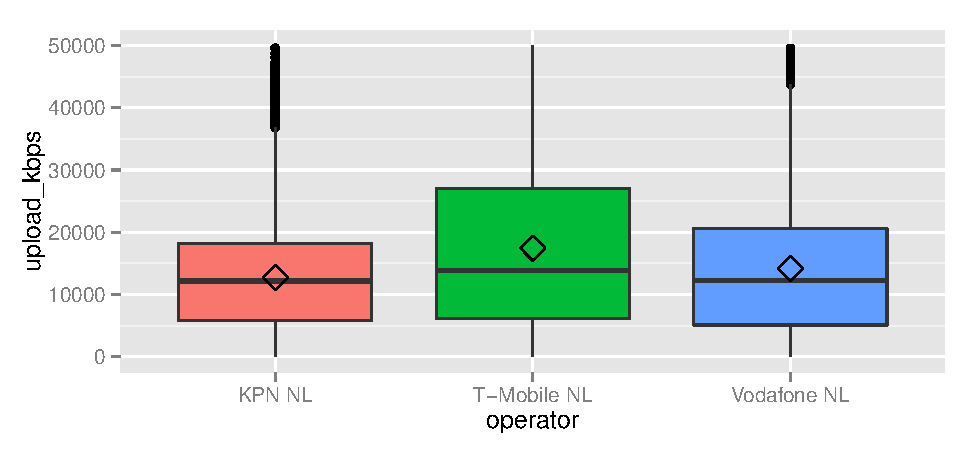
\includegraphics{speedtest-analysis_files/figure-latex/box-up-1.pdf}

Also in the box-plot we see that for T-Mobile the diamond shape(average)
and the thick line representing the median are higher then the same
values for the other operators. So also in this box-plot for upload
speed we see that T-Mobile has the highest average and median upload
speed.

If we zoom in on percentiles we can look at the fastest 10\%, 5\% and
1\% of speed tests:

\begin{longtable}[c]{@{}lrrr@{}}
\caption{Top percentiles average upload speed(Kbps)}\tabularnewline
\toprule
operator & 10\% & 5\% & 1\%\tabularnewline
\midrule
\endfirsthead
\toprule
operator & 10\% & 5\% & 1\%\tabularnewline
\midrule
\endhead
KPN NL & 21043 & 28200 & 42945\tabularnewline
T-Mobile NL & 39097 & 44205 & 46896\tabularnewline
Vodafone NL & 29486 & 39893 & 46296\tabularnewline
\bottomrule
\end{longtable}

From the table we see that T-Mobile scores best in the fastest 10\%,5\%
and 1\% of upload speed tests per operator.

\subsubsection{Latency}\label{latency-1}

For latency ( or ping) we take the log so the outliers scale and we can
have a look at the shape of the distribution.

We see a box plot for each of the operators on the x axis, the vertical
axis shows the speed test values in Kbps. The daimond shape represents
the mean, the thick line represents the median. the black dots on the
top and bottom represent extreme cases. The data is split up into
quartiles, that means four equally sized proportions. The first and
fourth quarter are represented as a line, the second and third as a box.

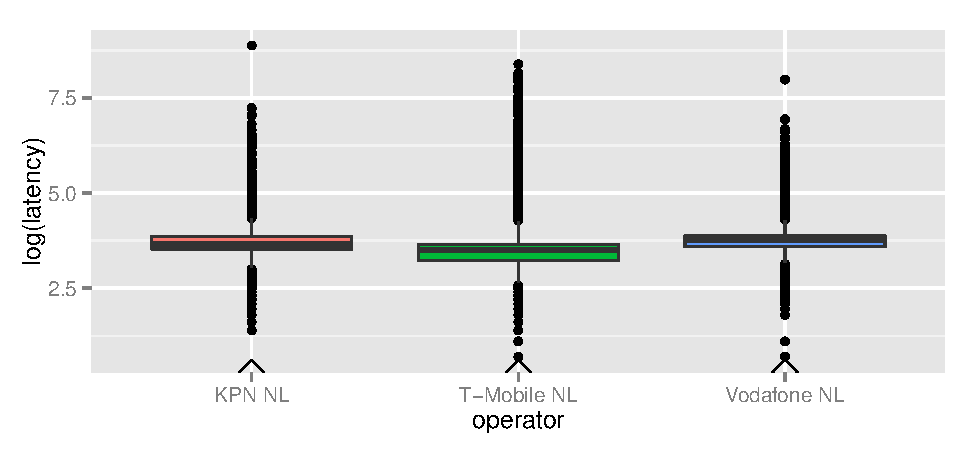
\includegraphics{speedtest-analysis_files/figure-latex/box-latency-1.pdf}

In the box-plot for latancy we see that for T-Mobile the diamond
shape(average) and the thick line representing the median are lower then
the same values for the other operators. Remember, for latancy lower is
better. So in this box-plot for latency we see that T-Mobile has the
lowest latency.

\newpage

\section{Step 4: Test design}\label{step-4-test-design}

What we want to test is if, on average, a customer that uses T-Mobile 4G
Mobile Network gets a higher average speed(in terms of download speed,
upload speed and latency) than a customer using KPN's or Vodafone's 4G
Mobile Network, with all else equal. To do this we have collected
thousands of Ookla NetMetrics Speedtest results taken from the three top
operators (KPN, Vodafone and T-Mobile) which have been filtered as set
out in the above to a final dataset consisting of 97749 data points. Now
we want to compare T-Mobile with the other two operators. So we do two
tests: the first is comparing T-Mobile with KPN and the second is
comparing T-Mobile with Vodafone. In each test we compare all three
metrics: Upload speed, Download speed and latency(or ping). For each
operator we have a sample set available in the data. These sets are so
called samples (from the Dutch population of mobile phone users) from
which we calculate the sample means. Now our statistical test tests if
these sample means are significantly different from one another.

In practice, the Central Limit Theorem assures us that, under a wide
range of assumptions, the distributions of the two sample means being
tested will themselves approach Normal distributions as the sample sizes
get large, regardless (this is where the assumptions come in) of the
distributions of the underlying data. As a consequence, as the sample
size gets larger, the difference of the means becomes normally
distributed, and the requirements necessary for the t-statistic of an
unpaired t-test to have the nominal t distribution become satisfied.

\subsection{Which statistical test do we
need?}\label{which-statistical-test-do-we-need}

What we have here is a set of unpaired, independent, different sample
size, different variance data. A suitable and powerful test for this
kind of data is a
\href{https://en.wikipedia.org/wiki/Welch\%27s_t_test}{Welch t-test}.

In statistics, Welch's t-test (or Welch-Aspin Test) is a two-sample
location test, and is used to check the hypothesis that two populations
have equal means(our NULL hypothesis). Welch's t-test is an adaptation
of Student's t-test, and is intended for use when the two samples have
possibly unequal variances(which is the case here). These tests are
often referred to as ``unpaired'' or ``independent samples'' t-tests, as
they are typically applied when the statistical units underlying the two
samples being compared are non-overlapping(in our case the units are
different people performing the test with different devices on different
networks).

\subsubsection{Significance}\label{significance}

So when is a test significant? And if so at what level? And furthermore
can we qualify such a significant result as good or bad? To start with
the last remark, all qualifications of a statistical result are
subjective. One way of looking at 95\% confidence is that 1 out of 20
trials (in 5\% of the cases) you make a so called Type 1 error, in which
you wrongly reject the null-hypothesis. So in this case, if the p-value
would be 0.05(confidence level 95\%) you would claim that operator x is
faster then operator y while in fact they were not. In applied practice,
confidence intervals are typically stated at the 95\% or 99\% confidence
level (More on
\href{https://en.wikipedia.org/wiki/Statistical_significance}{significance}
).

In our test we will set the confidence level to be 99\%, which is more
strict then 95\%. This means we will reject the Null Hypothesis only if
we are 99 \% confident we do not make a mistake. From the test result we
see that in most cases the calculated p-values are very much smaller
then 1 - 0.99 = 0.01, so changes of making this type of error are even
considerably smaller than the claimed confidence level of 99\%.

\subsubsection{P-value}\label{p-value}

In statistics, the p-value is a function of the observed sample results
(a statistic) that is used for testing a statistical hypothesis. Before
performing the test a threshold value is chosen, called the significance
level of the test, traditionally 5\% or 1\% and denoted as \(\alpha\).
If the p-value is equal or smaller than the significance level
(\(\alpha\)), it suggests that the observed data is inconsistent with
the assumption that the null hypothesis is true, and thus that
hypothesis must be rejected and the alternative hypothesis is accepted
as true ( see \href{https://en.wikipedia.org/wiki/P-value}{wikipedia}).

\subsubsection{Confidence intervals}\label{confidence-intervals}

Confidence intervals consist of a range of values (interval) that act as
good estimates of the unknown population parameter. The level of
confidence of the confidence interval would indicate the probability
that the confidence range captures this true population parameter given
a distribution of samples. This value is represented by a percentage, so
when we say, ``we are 99\% confident that the true value of the
parameter is in our confidence interval'', we express that 99\% of the
observed confidence intervals will hold the true value of the parameter.
A confidence interval does \textbf{not} predict that the true value of
the parameter has a particular probability of being in the confidence
interval given the data actually obtained. (see
\href{https://en.wikipedia.org/wiki/Confidence_interval}{wikipedia}).

\newpage

\section{Step 5: Test results coverage
area}\label{step-5-test-results-coverage-area}

We test T-Mobile against the other two operators so we have two tests.
We put the confidence level to 99 \%. Our null-hypothesis is that the
means are drawn from the same sample, so they are not different.

In this test we use the whole cleaned data set, in the next chapter we
test each individual city.

Let's see what our test results are:

\begin{table}[ht]
\centering
{\footnotesize
\begin{tabular}{lllllllllll}
  \hline
Operator1 & Operator2 & Sample1 & Mean1 & Sample2 & Mean2 & P-value & Sign. & Diff(Kbps) & Conf Int & Rel(\%) \\ 
  \hline
T-Mobile & KPN & 33225 & 40253 & 38164 & 28226 & $<$ 2.22e-16 & Yes & 12027 & +/- 467.9 & 42.6 \\ 
  T-Mobile & Vodafone & 33225 & 40253 & 26360 & 30106 & $<$ 2.22e-16 & Yes & 10147 & +/- 541.6 & 33.7 \\ 
   \hline
\end{tabular}
}
\caption{Comparison of means for metric: download(kbps)} 
\end{table}\begin{table}[ht]
\centering
{\footnotesize
\begin{tabular}{lllllllllll}
  \hline
Operator1 & Operator2 & Sample1 & Mean1 & Sample2 & Mean2 & P-value & Sign. & Diff(Kbps) & Conf Int & Rel(\%) \\ 
  \hline
T-Mobile & KPN & 33225 & 17443 & 38164 & 12728 & $<$ 2.22e-16 & Yes & 4715 & +/- 222.2 & 37 \\ 
  T-Mobile & Vodafone & 33225 & 17443 & 26360 & 14145 & $<$ 2.22e-16 & Yes & 3298 & +/- 260.9 & 23.3 \\ 
   \hline
\end{tabular}
}
\caption{Comparison of means for metric: upload(kbps)} 
\end{table}\begin{table}[ht]
\centering
{\footnotesize
\begin{tabular}{lllllllllll}
  \hline
Operator1 & Operator2 & Sample1 & Mean1 & Sample2 & Mean2 & P-value & Sign. & Diff(ms) & Conf Int & Rel(\%) \\ 
  \hline
T-Mobile & KPN & 33225 & 38 & 38164 & 43 & $<$ 2.22e-16 & Yes & -5.1 & +/- 1.3 & -11.9 \\ 
  T-Mobile & Vodafone & 33225 & 38 & 26360 & 45 & $<$ 2.22e-16 & Yes & -7.6 & +/- 1.2 & -16.7 \\ 
   \hline
\end{tabular}
}
\caption{Comparison of means for metric: latency(ms)} 
\end{table}

\textbf{Explanation of terms}

\footnotesize

\textbf{Sample 1}: Number of speed test samples for operator 1.

\textbf{Sample 2}: Number of speed test samples for operator 2.

\textbf{Mean 1}: Average speed of speed tests for operator 1 in KBps. A
high number here means that this operator has a fast download(or upload)
speed. For the latency a high number means you have to wait longer to
contact webpages or servers.

\textbf{Mean 2}: Average speed of speed tests for operator 2 in KBps. A
high number here means that this operator has a fast download(or upload)
speed. For the latency a high number means you have to wait longer to
contact webpages or servers.

\textbf{P-value}: The test statistic, for more explanation see the
paragraph P-Value above

\textbf{Sign.}: Short for Significance. We compare the test statistic
with the predefined confidence level(0.99). `Yes' means the test is
significant, `No' means the test is not significant.``))

\textbf{Diff(in Kbps or ms)}: Difference of the means (DoM) is the
difference of Mean 1 and Mean 2(Mean 1 - Mean 2). For download and
upload speeds(Kbps) big positive number here means operator 1 has a
faster speed then operator 2. A big negative number means that operator
2 has a faster speed then operator 1. For latency(ms) this is the
opposite, because smaller is better.

\textbf{Conf Int}: Confidence interval consist of a range of values
(interval) that act as good estimate of the \emph{true} difference of
the mean. We are 99\% confident that the true value of the difference of
the mean is in our confidence interval.

\textbf{Rel(\%)}: Relative difference in percentage. It is calculated as
the difference of the mean divided by the slower of the two operators
average speed. If the difference is not significant(column Sign is No),
this column will state NA(Not Applicable). The comparison rules are
similar to what is explained in the Diff(in Kbps or ms).

\normalsize
Looking at the tables above we see that all results are significant at
\(\alpha\) = 0.01 level(99\% confidence level) and the resulting
p-values are very small. This means we can reject the null-hypothesis
with great confidence. Hence we can state that with 99\% confidence the
true difference in the means lies within the confidence interval
provided in the table.

\newpage

\section{Conclusion}\label{conclusion}

This analysis has been conducted with the utmost care and to the best
knowledge of the analyst (DIKW Consulting). The analysis is opensource
and all code can be downloaded, reviewed and repeated from
\href{https://github.com/hugokoopmans/ookla-speedtest-analysis}{GitHub}.

Overall we can say that based on the speedtest data analysed in the
investigated area the 4G network of T-Mobile outperforms both KPN and
Vodafone on download speed, upload speed and latency.

From the data analysed in the investigated area the average download
speed of the 4G network of T-Mobile outperforms KPN by 12.03 Mbps, which
is 42.6\%. Also, from the data analysed in the investigated area the
average download speed of the 4G network of T-Mobile outperforms
Vodafone by 10.15 Mbps, which is 33.7\%. From table 14 above similar
statements can be derived for upload speed. For deriving these
statements for latency, please see table 15 keeping in mind that smaller
values are better.

For conclusions per individual city we refer to the section below.
Please keep in mind that the significance of a test per city does not
influence the significance of a test over the whole 4G area. The
significance of a test per city only shows if the 4G network speeds
(download speed, upload speed and latency) are also significantly
different on a local level, so for that city treated separately.

\newpage

\section{Analysis and results Top 21 cities per
city}\label{analysis-and-results-top-21-cities-per-city}

From CBS we have the following top 21 cities based on number of
inhabitants(``aantal inwoners'') from 2014. We see that Zwolle is now
number twenty in favour of Maastricht(now 21). For completness we keep
Maastricht in the list of cities to be analysed.

\begin{longtable}[c]{@{}llrr@{}}
\toprule
gm\_code & gm\_naam & aant\_inw & opp\_land\tabularnewline
\midrule
\endhead
GM0363 & Amsterdam & 810935 & 16589\tabularnewline
GM0599 & Rotterdam & 618355 & 20888\tabularnewline
GM0518 & 's-Gravenhage & 508940 & 8187\tabularnewline
GM0344 & Utrecht & 328165 & 9426\tabularnewline
GM0772 & Eindhoven & 220920 & 8767\tabularnewline
GM0855 & Tilburg & 210270 & 11724\tabularnewline
GM0014 & Groningen & 198315 & 7827\tabularnewline
GM0034 & Almere & 196010 & 12930\tabularnewline
GM0758 & Breda & 179620 & 12605\tabularnewline
GM0268 & Nijmegen & 168290 & 5361\tabularnewline
GM0153 & Enschede & 158585 & 14099\tabularnewline
GM0200 & Apeldoorn & 157545 & 33988\tabularnewline
GM0392 & Haarlem & 155145 & 2922\tabularnewline
GM0307 & Amersfoort & 150895 & 6282\tabularnewline
GM0202 & Arnhem & 150820 & 9796\tabularnewline
GM0479 & Zaanstad & 150595 & 7392\tabularnewline
GM0394 & Haarlemmermeer & 144060 & 17868\tabularnewline
GM0796 & 's-Hertogenbosch & 143730 & 8440\tabularnewline
GM0637 & Zoetermeer & 123560 & 3453\tabularnewline
GM0193 & Zwolle & 123160 & 11131\tabularnewline
GM0935 & Maastricht & 122485 & 5662\tabularnewline
\bottomrule
\end{longtable}

In this test we use the CBS cities in this area as the benchmark area
for the overall comparison.

In more detailed analysis we investigate the top twenty ``Gemeentes''
based on number of inhabitants. based on data available at
\href{http://www.cbs.nl/nl-NL/menu/themas/dossiers/nederland-regionaal/publicaties/geografische-data/archief/2014/2013-wijk-en-buurtkaart-art.htm}{CBS}.

The coverage area of top 20 cities looks like this.

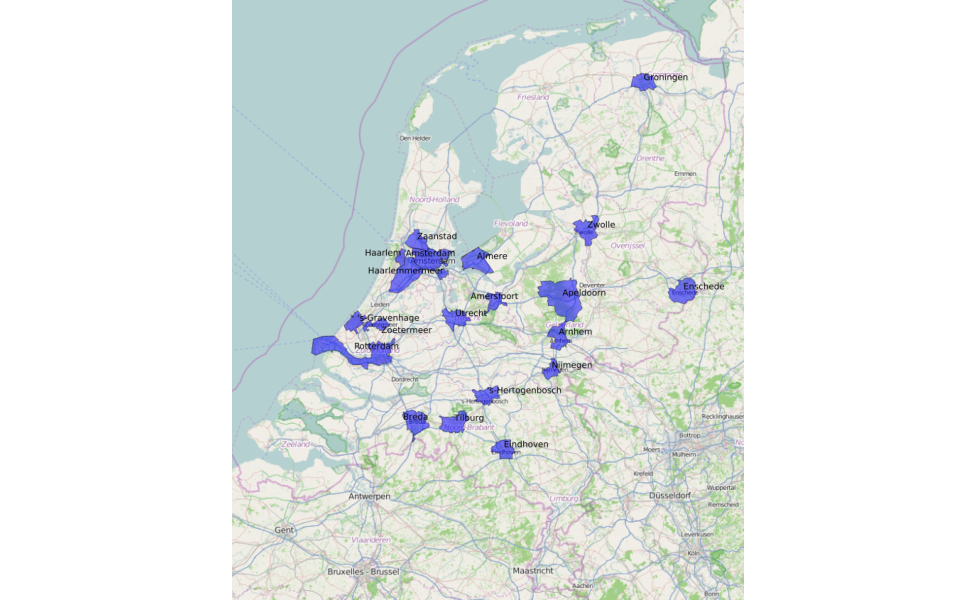
\includegraphics{speedtest-analysis_files/figure-latex/top-1.pdf}

From the CBS data we learn that the top 21 cities covers 5020400 out of
16828900 inhabitants. Which is 29.83 \%. In terms of area this is 235337
km\^{}2 of a total of 41545 km\^{}2, which is 566.46\%.

For each city we will do the significance test separately in the next
pages.

\newpage

\subsection{Gemeente Amsterdam}\label{gemeente-amsterdam}

The table shows the speed test analysis for gemeente Amsterdam. For this
test the confidence level is set to 99\%.

\begin{table}[ht]
\centering
{\footnotesize
\begin{tabular}{lllllllllll}
  \hline
Operator1 & Operator2 & Sample1 & Mean1 & Sample2 & Mean2 & P-value & Sign. & Diff(Kbps) & Conf Int & Rel(\%) \\ 
  \hline
T-Mobile & KPN & 5012 & 42288 & 2672 & 31822 & $<$ 2.22e-16 & Yes & 10466.4 & +/- 1687.5 & 32.9 \\ 
  T-Mobile & Vodafone & 5012 & 42288 & 2890 & 38652 & 5.4369e-08 & Yes & 3635.7 & +/- 1720.9 & 9.4 \\ 
   \hline
\end{tabular}
}
\caption{Comparison of means for metric: download(kbps)} 
\end{table}\begin{table}[ht]
\centering
{\footnotesize
\begin{tabular}{lllllllllll}
  \hline
Operator1 & Operator2 & Sample1 & Mean1 & Sample2 & Mean2 & P-value & Sign. & Diff(Kbps) & Conf Int & Rel(\%) \\ 
  \hline
T-Mobile & KPN & 5012 & 18904 & 2672 & 13439 & $<$ 2.22e-16 & Yes & 5465.1 & +/- 707.6 & 40.7 \\ 
  T-Mobile & Vodafone & 5012 & 18904 & 2890 & 16992 & 1.4466e-09 & Yes & 1912.2 & +/- 813.2 & 11.3 \\ 
   \hline
\end{tabular}
}
\caption{Comparison of means for metric: upload(kbps)} 
\end{table}\begin{table}[ht]
\centering
{\footnotesize
\begin{tabular}{lllllllllll}
  \hline
Operator1 & Operator2 & Sample1 & Mean1 & Sample2 & Mean2 & P-value & Sign. & Diff(ms) & Conf Int & Rel(\%) \\ 
  \hline
T-Mobile & KPN & 5012 & 34 & 2672 & 41 & 3.226e-09 & Yes & -6.7 & +/- 2.9 & -16.5 \\ 
  T-Mobile & Vodafone & 5012 & 34 & 2890 & 42 & 6.8797e-14 & Yes & -7.5 & +/- 2.6 & -18.1 \\ 
   \hline
\end{tabular}
}
\caption{Comparison of means for metric: latency(ms)} 
\end{table}

Please note the column {[}Sign.{]} or ``Significant'', if this column
states ``No'' the test is not significant at the 99\% confidence level.
This means there is no significant difference in means observed so the
NULL Hypothesis can not be rejected. In layman's terms: You
\emph{cannot} conclude that one operator has a faster 4G network then
the other on that particular 4G network speed measurement (download
speed, upload speed or latency).

\textbf{Explanation of terms}

\footnotesize

\textbf{Sample 1}: Number of speedtest samples for operator 1.

\textbf{Sample 2}: Number of speedtest samples for operator 2.

\textbf{Mean 1}: Average speed of speedtests for operator 1 in KBps. A
high number here means that this operator has a fast download(or upload)
speed. For the latency a high number means you have to wait longer to
contact webpages or servers.

\textbf{Mean 2}: Average speed of speedtests for operator 2 in KBps. A
high number here means that this operator has a fast download(or upload)
speed. For the latency a high number means you have to wait longer to
contact webpages or servers.

\textbf{P-value}: The test statistic, for more explanation see the
paragraph P-Value above

\textbf{Sign.}: Short for Significance. We compare the test statistic
with the predefined confidence level(0.99). `Yes' means the test is
significant, `No' means the test is not significant.``))

\textbf{Diff(in Kbps or ms)}: Difference of the means (DoM) is the
difference of Mean 1 and Mean 2(Mean 1 - Mean 2). For download and
upload speeds(Kbps) big positive number here means operator 1 has a
faster speed then operator 2. A big negative number means that operator
2 has a faster speed then operator 1. For latency(ms) this is the
opposite, because smaller is better.

\textbf{Conf Int}: Confidence interval consist of a range of values
(interval) that act as good estimate of the \emph{true} difference of
the mean. We are 99\% confident that the true value of the difference of
the mean is in our confidence interval.

\textbf{Rel(\%)}: Relative difference in percentage. It is calculated as
the difference of the mean divided by the slower of the two operators
average speed. If the difference is not significant (colums Sign is No),
this column will state NA (not applicable). The comparison rules are
similar to what is explained in the Diff(in Kbps or ms).

\normalsize

\newpage

\subsection{Gemeente Rotterdam}\label{gemeente-rotterdam}

The table shows the speed test analysis for gemeente Rotterdam. For this
test the confidence level is set to 99\%.

\begin{table}[ht]
\centering
{\footnotesize
\begin{tabular}{lllllllllll}
  \hline
Operator1 & Operator2 & Sample1 & Mean1 & Sample2 & Mean2 & P-value & Sign. & Diff(Kbps) & Conf Int & Rel(\%) \\ 
  \hline
T-Mobile & KPN & 2401 & 39498 & 2025 & 35780 & 2.3722e-06 & Yes & 3718.3 & +/- 2027.8 & 10.4 \\ 
  T-Mobile & Vodafone & 2401 & 39498 & 1382 & 39046 & 0.6408 & No & 452.2 & +/- 2498.2 & NA \\ 
   \hline
\end{tabular}
}
\caption{Comparison of means for metric: download(kbps)} 
\end{table}\begin{table}[ht]
\centering
{\footnotesize
\begin{tabular}{lllllllllll}
  \hline
Operator1 & Operator2 & Sample1 & Mean1 & Sample2 & Mean2 & P-value & Sign. & Diff(Kbps) & Conf Int & Rel(\%) \\ 
  \hline
T-Mobile & KPN & 2401 & 19390 & 2025 & 15013 & $<$ 2.22e-16 & Yes & 4377.1 & +/- 933.1 & 29.2 \\ 
  T-Mobile & Vodafone & 2401 & 19390 & 1382 & 17622 & 9.5404e-05 & Yes & 1768.1 & +/- 1166.3 & 10 \\ 
   \hline
\end{tabular}
}
\caption{Comparison of means for metric: upload(kbps)} 
\end{table}\begin{table}[ht]
\centering
{\footnotesize
\begin{tabular}{lllllllllll}
  \hline
Operator1 & Operator2 & Sample1 & Mean1 & Sample2 & Mean2 & P-value & Sign. & Diff(ms) & Conf Int & Rel(\%) \\ 
  \hline
T-Mobile & KPN & 2401 & 37 & 2025 & 41 & 0.0082147 & Yes & -4.2 & +/- 4.1 & -10.1 \\ 
  T-Mobile & Vodafone & 2401 & 37 & 1382 & 43 & 0.00017652 & Yes & -6 & +/- 4.1 & -13.9 \\ 
   \hline
\end{tabular}
}
\caption{Comparison of means for metric: latency(ms)} 
\end{table}

Please note the column {[}Sign.{]} or ``Significant'', if this column
states ``No'' the test is not significant at the 99\% confidence level.
This means there is no significant difference in means observed so the
NULL Hypothesis can not be rejected. In layman's terms: You
\emph{cannot} conclude that one operator has a faster 4G network then
the other on that particular 4G network speed measurement (download
speed, upload speed or latency).

\textbf{Explanation of terms}

\footnotesize

\textbf{Sample 1}: Number of speedtest samples for operator 1.

\textbf{Sample 2}: Number of speedtest samples for operator 2.

\textbf{Mean 1}: Average speed of speedtests for operator 1 in KBps. A
high number here means that this operator has a fast download(or upload)
speed. For the latency a high number means you have to wait longer to
contact webpages or servers.

\textbf{Mean 2}: Average speed of speedtests for operator 2 in KBps. A
high number here means that this operator has a fast download(or upload)
speed. For the latency a high number means you have to wait longer to
contact webpages or servers.

\textbf{P-value}: The test statistic, for more explanation see the
paragraph P-Value above

\textbf{Sign.}: Short for Significance. We compare the test statistic
with the predefined confidence level(0.99). `Yes' means the test is
significant, `No' means the test is not significant.``))

\textbf{Diff(in Kbps or ms)}: Difference of the means (DoM) is the
difference of Mean 1 and Mean 2(Mean 1 - Mean 2). For download and
upload speeds(Kbps) big positive number here means operator 1 has a
faster speed then operator 2. A big negative number means that operator
2 has a faster speed then operator 1. For latency(ms) this is the
opposite, because smaller is better.

\textbf{Conf Int}: Confidence interval consist of a range of values
(interval) that act as good estimate of the \emph{true} difference of
the mean. We are 99\% confident that the true value of the difference of
the mean is in our confidence interval.

\textbf{Rel(\%)}: Relative difference in percentage. It is calculated as
the difference of the mean divided by the slower of the two operators
average speed. If the difference is not significant (colums Sign is No),
this column will state NA (not applicable). The comparison rules are
similar to what is explained in the Diff(in Kbps or ms).

\normalsize

\newpage

\subsection{Gemeente 's-Gravenhage}\label{gemeente-s-gravenhage}

The table shows the speed test analysis for gemeente 's-Gravenhage. For
this test the confidence level is set to 99\%.

\begin{table}[ht]
\centering
{\footnotesize
\begin{tabular}{lllllllllll}
  \hline
Operator1 & Operator2 & Sample1 & Mean1 & Sample2 & Mean2 & P-value & Sign. & Diff(Kbps) & Conf Int & Rel(\%) \\ 
  \hline
T-Mobile & KPN & 1893 & 39992 & 2280 & 33708 & 4.7325e-15 & Yes & 6283.9 & +/- 2059.4 & 18.6 \\ 
  T-Mobile & Vodafone & 1893 & 39992 & 1177 & 36044 & 0.00010084 & Yes & 3947.5 & +/- 2612.4 & 11 \\ 
   \hline
\end{tabular}
}
\caption{Comparison of means for metric: download(kbps)} 
\end{table}\begin{table}[ht]
\centering
{\footnotesize
\begin{tabular}{lllllllllll}
  \hline
Operator1 & Operator2 & Sample1 & Mean1 & Sample2 & Mean2 & P-value & Sign. & Diff(Kbps) & Conf Int & Rel(\%) \\ 
  \hline
T-Mobile & KPN & 1893 & 20207 & 2280 & 15155 & $<$ 2.22e-16 & Yes & 5051.3 & +/- 995.4 & 33.3 \\ 
  T-Mobile & Vodafone & 1893 & 20207 & 1177 & 15369 & $<$ 2.22e-16 & Yes & 4838.2 & +/- 1296.8 & 31.5 \\ 
   \hline
\end{tabular}
}
\caption{Comparison of means for metric: upload(kbps)} 
\end{table}\begin{table}[ht]
\centering
{\footnotesize
\begin{tabular}{lllllllllll}
  \hline
Operator1 & Operator2 & Sample1 & Mean1 & Sample2 & Mean2 & P-value & Sign. & Diff(ms) & Conf Int & Rel(\%) \\ 
  \hline
T-Mobile & KPN & 1893 & 38 & 2280 & 43 & 0.16349 & No & -4.5 & +/- 8.3 & NA \\ 
  T-Mobile & Vodafone & 1893 & 38 & 1177 & 47 & 0.0090452 & Yes & -8.4 & +/- 8.3 & -17.9 \\ 
   \hline
\end{tabular}
}
\caption{Comparison of means for metric: latency(ms)} 
\end{table}

Please note the column {[}Sign.{]} or ``Significant'', if this column
states ``No'' the test is not significant at the 99\% confidence level.
This means there is no significant difference in means observed so the
NULL Hypothesis can not be rejected. In layman's terms: You
\emph{cannot} conclude that one operator has a faster 4G network then
the other on that particular 4G network speed measurement (download
speed, upload speed or latency).

\textbf{Explanation of terms}

\footnotesize

\textbf{Sample 1}: Number of speedtest samples for operator 1.

\textbf{Sample 2}: Number of speedtest samples for operator 2.

\textbf{Mean 1}: Average speed of speedtests for operator 1 in KBps. A
high number here means that this operator has a fast download(or upload)
speed. For the latency a high number means you have to wait longer to
contact webpages or servers.

\textbf{Mean 2}: Average speed of speedtests for operator 2 in KBps. A
high number here means that this operator has a fast download(or upload)
speed. For the latency a high number means you have to wait longer to
contact webpages or servers.

\textbf{P-value}: The test statistic, for more explanation see the
paragraph P-Value above

\textbf{Sign.}: Short for Significance. We compare the test statistic
with the predefined confidence level(0.99). `Yes' means the test is
significant, `No' means the test is not significant.``))

\textbf{Diff(in Kbps or ms)}: Difference of the means (DoM) is the
difference of Mean 1 and Mean 2(Mean 1 - Mean 2). For download and
upload speeds(Kbps) big positive number here means operator 1 has a
faster speed then operator 2. A big negative number means that operator
2 has a faster speed then operator 1. For latency(ms) this is the
opposite, because smaller is better.

\textbf{Conf Int}: Confidence interval consist of a range of values
(interval) that act as good estimate of the \emph{true} difference of
the mean. We are 99\% confident that the true value of the difference of
the mean is in our confidence interval.

\textbf{Rel(\%)}: Relative difference in percentage. It is calculated as
the difference of the mean divided by the slower of the two operators
average speed. If the difference is not significant (colums Sign is No),
this column will state NA (not applicable). The comparison rules are
similar to what is explained in the Diff(in Kbps or ms).

\normalsize

\newpage

\subsection{Gemeente Utrecht}\label{gemeente-utrecht}

The table shows the speed test analysis for gemeente Utrecht. For this
test the confidence level is set to 99\%.

\begin{table}[ht]
\centering
{\footnotesize
\begin{tabular}{lllllllllll}
  \hline
Operator1 & Operator2 & Sample1 & Mean1 & Sample2 & Mean2 & P-value & Sign. & Diff(Kbps) & Conf Int & Rel(\%) \\ 
  \hline
T-Mobile & KPN & 1045 & 37675 & 1377 & 33289 & 4.5912e-05 & Yes & 4385.9 & +/- 2769 & 13.2 \\ 
  T-Mobile & Vodafone & 1045 & 37675 & 1047 & 37923 & 0.83063 & No & -248 & +/- 2988.5 & NA \\ 
   \hline
\end{tabular}
}
\caption{Comparison of means for metric: download(kbps)} 
\end{table}\begin{table}[ht]
\centering
{\footnotesize
\begin{tabular}{lllllllllll}
  \hline
Operator1 & Operator2 & Sample1 & Mean1 & Sample2 & Mean2 & P-value & Sign. & Diff(Kbps) & Conf Int & Rel(\%) \\ 
  \hline
T-Mobile & KPN & 1045 & 18067 & 1377 & 15024 & 7.217e-10 & Yes & 3043.6 & +/- 1266.9 & 20.3 \\ 
  T-Mobile & Vodafone & 1045 & 18067 & 1047 & 16551 & 0.0083012 & Yes & 1516.6 & +/- 1479.9 & 9.2 \\ 
   \hline
\end{tabular}
}
\caption{Comparison of means for metric: upload(kbps)} 
\end{table}\begin{table}[ht]
\centering
{\footnotesize
\begin{tabular}{lllllllllll}
  \hline
Operator1 & Operator2 & Sample1 & Mean1 & Sample2 & Mean2 & P-value & Sign. & Diff(ms) & Conf Int & Rel(\%) \\ 
  \hline
T-Mobile & KPN & 1045 & 36 & 1377 & 42 & 0.00011519 & Yes & -5.8 & +/- 3.9 & -13.7 \\ 
  T-Mobile & Vodafone & 1045 & 36 & 1047 & 42 & 0.00014179 & Yes & -5.9 & +/- 4 & -13.9 \\ 
   \hline
\end{tabular}
}
\caption{Comparison of means for metric: latency(ms)} 
\end{table}

Please note the column {[}Sign.{]} or ``Significant'', if this column
states ``No'' the test is not significant at the 99\% confidence level.
This means there is no significant difference in means observed so the
NULL Hypothesis can not be rejected. In layman's terms: You
\emph{cannot} conclude that one operator has a faster 4G network then
the other on that particular 4G network speed measurement (download
speed, upload speed or latency).

\textbf{Explanation of terms}

\footnotesize

\textbf{Sample 1}: Number of speedtest samples for operator 1.

\textbf{Sample 2}: Number of speedtest samples for operator 2.

\textbf{Mean 1}: Average speed of speedtests for operator 1 in KBps. A
high number here means that this operator has a fast download(or upload)
speed. For the latency a high number means you have to wait longer to
contact webpages or servers.

\textbf{Mean 2}: Average speed of speedtests for operator 2 in KBps. A
high number here means that this operator has a fast download(or upload)
speed. For the latency a high number means you have to wait longer to
contact webpages or servers.

\textbf{P-value}: The test statistic, for more explanation see the
paragraph P-Value above

\textbf{Sign.}: Short for Significance. We compare the test statistic
with the predefined confidence level(0.99). `Yes' means the test is
significant, `No' means the test is not significant.``))

\textbf{Diff(in Kbps or ms)}: Difference of the means (DoM) is the
difference of Mean 1 and Mean 2(Mean 1 - Mean 2). For download and
upload speeds(Kbps) big positive number here means operator 1 has a
faster speed then operator 2. A big negative number means that operator
2 has a faster speed then operator 1. For latency(ms) this is the
opposite, because smaller is better.

\textbf{Conf Int}: Confidence interval consist of a range of values
(interval) that act as good estimate of the \emph{true} difference of
the mean. We are 99\% confident that the true value of the difference of
the mean is in our confidence interval.

\textbf{Rel(\%)}: Relative difference in percentage. It is calculated as
the difference of the mean divided by the slower of the two operators
average speed. If the difference is not significant (colums Sign is No),
this column will state NA (not applicable). The comparison rules are
similar to what is explained in the Diff(in Kbps or ms).

\normalsize

\newpage

\subsection{Gemeente Eindhoven}\label{gemeente-eindhoven}

The table shows the speed test analysis for gemeente Eindhoven. For this
test the confidence level is set to 99\%.

\begin{table}[ht]
\centering
{\footnotesize
\begin{tabular}{lllllllllll}
  \hline
Operator1 & Operator2 & Sample1 & Mean1 & Sample2 & Mean2 & P-value & Sign. & Diff(Kbps) & Conf Int & Rel(\%) \\ 
  \hline
T-Mobile & KPN & 744 & 41539 & 858 & 39485 & 0.12189 & No & 2053.8 & +/- 3422.2 & NA \\ 
  T-Mobile & Vodafone & 744 & 41539 & 842 & 33202 & 3.6011e-10 & Yes & 8336.1 & +/- 3406.5 & 25.1 \\ 
   \hline
\end{tabular}
}
\caption{Comparison of means for metric: download(kbps)} 
\end{table}\begin{table}[ht]
\centering
{\footnotesize
\begin{tabular}{lllllllllll}
  \hline
Operator1 & Operator2 & Sample1 & Mean1 & Sample2 & Mean2 & P-value & Sign. & Diff(Kbps) & Conf Int & Rel(\%) \\ 
  \hline
T-Mobile & KPN & 744 & 18622 & 858 & 16655 & 0.0013471 & Yes & 1967.1 & +/- 1579.6 & 11.8 \\ 
  T-Mobile & Vodafone & 744 & 18622 & 842 & 15610 & 6.7048e-07 & Yes & 3012 & +/- 1556.4 & 19.3 \\ 
   \hline
\end{tabular}
}
\caption{Comparison of means for metric: upload(kbps)} 
\end{table}\begin{table}[ht]
\centering
{\footnotesize
\begin{tabular}{lllllllllll}
  \hline
Operator1 & Operator2 & Sample1 & Mean1 & Sample2 & Mean2 & P-value & Sign. & Diff(ms) & Conf Int & Rel(\%) \\ 
  \hline
T-Mobile & KPN & 744 & 41 & 858 & 44 & 0.48571 & No & -2.6 & +/- 9.7 & NA \\ 
  T-Mobile & Vodafone & 744 & 41 & 842 & 49 & 0.031328 & No & -8.2 & +/- 9.8 & NA \\ 
   \hline
\end{tabular}
}
\caption{Comparison of means for metric: latency(ms)} 
\end{table}

Please note the column {[}Sign.{]} or ``Significant'', if this column
states ``No'' the test is not significant at the 99\% confidence level.
This means there is no significant difference in means observed so the
NULL Hypothesis can not be rejected. In layman's terms: You
\emph{cannot} conclude that one operator has a faster 4G network then
the other on that particular 4G network speed measurement (download
speed, upload speed or latency).

\textbf{Explanation of terms}

\footnotesize

\textbf{Sample 1}: Number of speedtest samples for operator 1.

\textbf{Sample 2}: Number of speedtest samples for operator 2.

\textbf{Mean 1}: Average speed of speedtests for operator 1 in KBps. A
high number here means that this operator has a fast download(or upload)
speed. For the latency a high number means you have to wait longer to
contact webpages or servers.

\textbf{Mean 2}: Average speed of speedtests for operator 2 in KBps. A
high number here means that this operator has a fast download(or upload)
speed. For the latency a high number means you have to wait longer to
contact webpages or servers.

\textbf{P-value}: The test statistic, for more explanation see the
paragraph P-Value above

\textbf{Sign.}: Short for Significance. We compare the test statistic
with the predefined confidence level(0.99). `Yes' means the test is
significant, `No' means the test is not significant.``))

\textbf{Diff(in Kbps or ms)}: Difference of the means (DoM) is the
difference of Mean 1 and Mean 2(Mean 1 - Mean 2). For download and
upload speeds(Kbps) big positive number here means operator 1 has a
faster speed then operator 2. A big negative number means that operator
2 has a faster speed then operator 1. For latency(ms) this is the
opposite, because smaller is better.

\textbf{Conf Int}: Confidence interval consist of a range of values
(interval) that act as good estimate of the \emph{true} difference of
the mean. We are 99\% confident that the true value of the difference of
the mean is in our confidence interval.

\textbf{Rel(\%)}: Relative difference in percentage. It is calculated as
the difference of the mean divided by the slower of the two operators
average speed. If the difference is not significant (colums Sign is No),
this column will state NA (not applicable). The comparison rules are
similar to what is explained in the Diff(in Kbps or ms).

\normalsize

\newpage

\subsection{Gemeente Tilburg}\label{gemeente-tilburg}

The table shows the speed test analysis for gemeente Tilburg. For this
test the confidence level is set to 99\%.

\begin{table}[ht]
\centering
{\footnotesize
\begin{tabular}{lllllllllll}
  \hline
Operator1 & Operator2 & Sample1 & Mean1 & Sample2 & Mean2 & P-value & Sign. & Diff(Kbps) & Conf Int & Rel(\%) \\ 
  \hline
T-Mobile & KPN & 486 & 40094 & 553 & 33659 & 6.9534e-05 & Yes & 6435.6 & +/- 4158 & 19.1 \\ 
  T-Mobile & Vodafone & 486 & 40094 & 346 & 32889 & 0.00040144 & Yes & 7205.7 & +/- 5232.1 & 21.9 \\ 
   \hline
\end{tabular}
}
\caption{Comparison of means for metric: download(kbps)} 
\end{table}\begin{table}[ht]
\centering
{\footnotesize
\begin{tabular}{lllllllllll}
  \hline
Operator1 & Operator2 & Sample1 & Mean1 & Sample2 & Mean2 & P-value & Sign. & Diff(Kbps) & Conf Int & Rel(\%) \\ 
  \hline
T-Mobile & KPN & 486 & 15941 & 553 & 14929 & 0.1689 & No & 1012.4 & +/- 1898.1 & NA \\ 
  T-Mobile & Vodafone & 486 & 15941 & 346 & 13871 & 0.014233 & No & 2069.9 & +/- 2175.5 & NA \\ 
   \hline
\end{tabular}
}
\caption{Comparison of means for metric: upload(kbps)} 
\end{table}\begin{table}[ht]
\centering
{\footnotesize
\begin{tabular}{lllllllllll}
  \hline
Operator1 & Operator2 & Sample1 & Mean1 & Sample2 & Mean2 & P-value & Sign. & Diff(ms) & Conf Int & Rel(\%) \\ 
  \hline
T-Mobile & KPN & 486 & 42 & 553 & 44 & 0.60324 & No & -1.9 & +/- 9.4 & NA \\ 
  T-Mobile & Vodafone & 486 & 42 & 346 & 48 & 0.11551 & No & -5.8 & +/- 9.5 & NA \\ 
   \hline
\end{tabular}
}
\caption{Comparison of means for metric: latency(ms)} 
\end{table}

Please note the column {[}Sign.{]} or ``Significant'', if this column
states ``No'' the test is not significant at the 99\% confidence level.
This means there is no significant difference in means observed so the
NULL Hypothesis can not be rejected. In layman's terms: You
\emph{cannot} conclude that one operator has a faster 4G network then
the other on that particular 4G network speed measurement (download
speed, upload speed or latency).

\textbf{Explanation of terms}

\footnotesize

\textbf{Sample 1}: Number of speedtest samples for operator 1.

\textbf{Sample 2}: Number of speedtest samples for operator 2.

\textbf{Mean 1}: Average speed of speedtests for operator 1 in KBps. A
high number here means that this operator has a fast download(or upload)
speed. For the latency a high number means you have to wait longer to
contact webpages or servers.

\textbf{Mean 2}: Average speed of speedtests for operator 2 in KBps. A
high number here means that this operator has a fast download(or upload)
speed. For the latency a high number means you have to wait longer to
contact webpages or servers.

\textbf{P-value}: The test statistic, for more explanation see the
paragraph P-Value above

\textbf{Sign.}: Short for Significance. We compare the test statistic
with the predefined confidence level(0.99). `Yes' means the test is
significant, `No' means the test is not significant.``))

\textbf{Diff(in Kbps or ms)}: Difference of the means (DoM) is the
difference of Mean 1 and Mean 2(Mean 1 - Mean 2). For download and
upload speeds(Kbps) big positive number here means operator 1 has a
faster speed then operator 2. A big negative number means that operator
2 has a faster speed then operator 1. For latency(ms) this is the
opposite, because smaller is better.

\textbf{Conf Int}: Confidence interval consist of a range of values
(interval) that act as good estimate of the \emph{true} difference of
the mean. We are 99\% confident that the true value of the difference of
the mean is in our confidence interval.

\textbf{Rel(\%)}: Relative difference in percentage. It is calculated as
the difference of the mean divided by the slower of the two operators
average speed. If the difference is not significant (colums Sign is No),
this column will state NA (not applicable). The comparison rules are
similar to what is explained in the Diff(in Kbps or ms).

\normalsize

\newpage

\subsection{Gemeente Groningen}\label{gemeente-groningen}

The table shows the speed test analysis for gemeente Groningen. For this
test the confidence level is set to 99\%.

\begin{table}[ht]
\centering
{\footnotesize
\begin{tabular}{lllllllllll}
  \hline
Operator1 & Operator2 & Sample1 & Mean1 & Sample2 & Mean2 & P-value & Sign. & Diff(Kbps) & Conf Int & Rel(\%) \\ 
  \hline
T-Mobile & KPN & 540 & 39799 & 894 & 33077 & 2.1557e-06 & Yes & 6721.4 & +/- 3641.8 & 20.3 \\ 
  T-Mobile & Vodafone & 540 & 39799 & 447 & 26705 & $<$ 2.22e-16 & Yes & 13093.4 & +/- 3967.2 & 49 \\ 
   \hline
\end{tabular}
}
\caption{Comparison of means for metric: download(kbps)} 
\end{table}\begin{table}[ht]
\centering
{\footnotesize
\begin{tabular}{lllllllllll}
  \hline
Operator1 & Operator2 & Sample1 & Mean1 & Sample2 & Mean2 & P-value & Sign. & Diff(Kbps) & Conf Int & Rel(\%) \\ 
  \hline
T-Mobile & KPN & 540 & 19883 & 894 & 13967 & 8.4047e-16 & Yes & 5916.4 & +/- 1859.7 & 42.4 \\ 
  T-Mobile & Vodafone & 540 & 19883 & 447 & 14326 & 9.8405e-12 & Yes & 5557 & +/- 2080.3 & 38.8 \\ 
   \hline
\end{tabular}
}
\caption{Comparison of means for metric: upload(kbps)} 
\end{table}\begin{table}[ht]
\centering
{\footnotesize
\begin{tabular}{lllllllllll}
  \hline
Operator1 & Operator2 & Sample1 & Mean1 & Sample2 & Mean2 & P-value & Sign. & Diff(ms) & Conf Int & Rel(\%) \\ 
  \hline
T-Mobile & KPN & 540 & 40 & 894 & 43 & 0.20309 & No & -2.5 & +/- 5.2 & NA \\ 
  T-Mobile & Vodafone & 540 & 40 & 447 & 46 & 0.0083408 & Yes & -5.3 & +/- 5.2 & -11.6 \\ 
   \hline
\end{tabular}
}
\caption{Comparison of means for metric: latency(ms)} 
\end{table}

Please note the column {[}Sign.{]} or ``Significant'', if this column
states ``No'' the test is not significant at the 99\% confidence level.
This means there is no significant difference in means observed so the
NULL Hypothesis can not be rejected. In layman's terms: You
\emph{cannot} conclude that one operator has a faster 4G network then
the other on that particular 4G network speed measurement (download
speed, upload speed or latency).

\textbf{Explanation of terms}

\footnotesize

\textbf{Sample 1}: Number of speedtest samples for operator 1.

\textbf{Sample 2}: Number of speedtest samples for operator 2.

\textbf{Mean 1}: Average speed of speedtests for operator 1 in KBps. A
high number here means that this operator has a fast download(or upload)
speed. For the latency a high number means you have to wait longer to
contact webpages or servers.

\textbf{Mean 2}: Average speed of speedtests for operator 2 in KBps. A
high number here means that this operator has a fast download(or upload)
speed. For the latency a high number means you have to wait longer to
contact webpages or servers.

\textbf{P-value}: The test statistic, for more explanation see the
paragraph P-Value above

\textbf{Sign.}: Short for Significance. We compare the test statistic
with the predefined confidence level(0.99). `Yes' means the test is
significant, `No' means the test is not significant.``))

\textbf{Diff(in Kbps or ms)}: Difference of the means (DoM) is the
difference of Mean 1 and Mean 2(Mean 1 - Mean 2). For download and
upload speeds(Kbps) big positive number here means operator 1 has a
faster speed then operator 2. A big negative number means that operator
2 has a faster speed then operator 1. For latency(ms) this is the
opposite, because smaller is better.

\textbf{Conf Int}: Confidence interval consist of a range of values
(interval) that act as good estimate of the \emph{true} difference of
the mean. We are 99\% confident that the true value of the difference of
the mean is in our confidence interval.

\textbf{Rel(\%)}: Relative difference in percentage. It is calculated as
the difference of the mean divided by the slower of the two operators
average speed. If the difference is not significant (colums Sign is No),
this column will state NA (not applicable). The comparison rules are
similar to what is explained in the Diff(in Kbps or ms).

\normalsize

\newpage

\subsection{Gemeente Almere}\label{gemeente-almere}

The table shows the speed test analysis for gemeente Almere. For this
test the confidence level is set to 99\%.

\begin{table}[ht]
\centering
{\footnotesize
\begin{tabular}{lllllllllll}
  \hline
Operator1 & Operator2 & Sample1 & Mean1 & Sample2 & Mean2 & P-value & Sign. & Diff(Kbps) & Conf Int & Rel(\%) \\ 
  \hline
T-Mobile & KPN & 413 & 40905 & 657 & 31310 & 5.4743e-09 & Yes & 9595 & +/- 4207 & 30.6 \\ 
  T-Mobile & Vodafone & 413 & 40905 & 393 & 28697 & 2.8881e-12 & Yes & 12207.4 & +/- 4443.9 & 42.5 \\ 
   \hline
\end{tabular}
}
\caption{Comparison of means for metric: download(kbps)} 
\end{table}\begin{table}[ht]
\centering
{\footnotesize
\begin{tabular}{lllllllllll}
  \hline
Operator1 & Operator2 & Sample1 & Mean1 & Sample2 & Mean2 & P-value & Sign. & Diff(Kbps) & Conf Int & Rel(\%) \\ 
  \hline
T-Mobile & KPN & 413 & 15041 & 657 & 13254 & 0.0093687 & Yes & 1786.4 & +/- 1770.9 & 13.5 \\ 
  T-Mobile & Vodafone & 413 & 15041 & 393 & 12455 & 0.0012006 & Yes & 2585.1 & +/- 2053.5 & 20.8 \\ 
   \hline
\end{tabular}
}
\caption{Comparison of means for metric: upload(kbps)} 
\end{table}\begin{table}[ht]
\centering
{\footnotesize
\begin{tabular}{lllllllllll}
  \hline
Operator1 & Operator2 & Sample1 & Mean1 & Sample2 & Mean2 & P-value & Sign. & Diff(ms) & Conf Int & Rel(\%) \\ 
  \hline
T-Mobile & KPN & 413 & 34 & 657 & 41 & 1.0081e-05 & Yes & -7.4 & +/- 4.3 & -18 \\ 
  T-Mobile & Vodafone & 413 & 34 & 393 & 43 & 2.5929e-07 & Yes & -9.6 & +/- 4.7 & -22.3 \\ 
   \hline
\end{tabular}
}
\caption{Comparison of means for metric: latency(ms)} 
\end{table}

Please note the column {[}Sign.{]} or ``Significant'', if this column
states ``No'' the test is not significant at the 99\% confidence level.
This means there is no significant difference in means observed so the
NULL Hypothesis can not be rejected. In layman's terms: You
\emph{cannot} conclude that one operator has a faster 4G network then
the other on that particular 4G network speed measurement (download
speed, upload speed or latency).

\textbf{Explanation of terms}

\footnotesize

\textbf{Sample 1}: Number of speedtest samples for operator 1.

\textbf{Sample 2}: Number of speedtest samples for operator 2.

\textbf{Mean 1}: Average speed of speedtests for operator 1 in KBps. A
high number here means that this operator has a fast download(or upload)
speed. For the latency a high number means you have to wait longer to
contact webpages or servers.

\textbf{Mean 2}: Average speed of speedtests for operator 2 in KBps. A
high number here means that this operator has a fast download(or upload)
speed. For the latency a high number means you have to wait longer to
contact webpages or servers.

\textbf{P-value}: The test statistic, for more explanation see the
paragraph P-Value above

\textbf{Sign.}: Short for Significance. We compare the test statistic
with the predefined confidence level(0.99). `Yes' means the test is
significant, `No' means the test is not significant.``))

\textbf{Diff(in Kbps or ms)}: Difference of the means (DoM) is the
difference of Mean 1 and Mean 2(Mean 1 - Mean 2). For download and
upload speeds(Kbps) big positive number here means operator 1 has a
faster speed then operator 2. A big negative number means that operator
2 has a faster speed then operator 1. For latency(ms) this is the
opposite, because smaller is better.

\textbf{Conf Int}: Confidence interval consist of a range of values
(interval) that act as good estimate of the \emph{true} difference of
the mean. We are 99\% confident that the true value of the difference of
the mean is in our confidence interval.

\textbf{Rel(\%)}: Relative difference in percentage. It is calculated as
the difference of the mean divided by the slower of the two operators
average speed. If the difference is not significant (colums Sign is No),
this column will state NA (not applicable). The comparison rules are
similar to what is explained in the Diff(in Kbps or ms).

\normalsize

\newpage

\subsection{Gemeente Breda}\label{gemeente-breda}

The table shows the speed test analysis for gemeente Breda. For this
test the confidence level is set to 99\%.

\begin{table}[ht]
\centering
{\footnotesize
\begin{tabular}{lllllllllll}
  \hline
Operator1 & Operator2 & Sample1 & Mean1 & Sample2 & Mean2 & P-value & Sign. & Diff(Kbps) & Conf Int & Rel(\%) \\ 
  \hline
T-Mobile & KPN & 487 & 40572 & 458 & 23860 & $<$ 2.22e-16 & Yes & 16712.1 & +/- 3311.6 & 70 \\ 
  T-Mobile & Vodafone & 487 & 40572 & 289 & 26606 & $<$ 2.22e-16 & Yes & 13965.8 & +/- 4113.2 & 52.5 \\ 
   \hline
\end{tabular}
}
\caption{Comparison of means for metric: download(kbps)} 
\end{table}\begin{table}[ht]
\centering
{\footnotesize
\begin{tabular}{lllllllllll}
  \hline
Operator1 & Operator2 & Sample1 & Mean1 & Sample2 & Mean2 & P-value & Sign. & Diff(Kbps) & Conf Int & Rel(\%) \\ 
  \hline
T-Mobile & KPN & 487 & 19933 & 458 & 10943 & $<$ 2.22e-16 & Yes & 8989.4 & +/- 1927.1 & 82.1 \\ 
  T-Mobile & Vodafone & 487 & 19933 & 289 & 12816 & 4.4583e-14 & Yes & 7116.9 & +/- 2388.4 & 55.5 \\ 
   \hline
\end{tabular}
}
\caption{Comparison of means for metric: upload(kbps)} 
\end{table}\begin{table}[ht]
\centering
{\footnotesize
\begin{tabular}{lllllllllll}
  \hline
Operator1 & Operator2 & Sample1 & Mean1 & Sample2 & Mean2 & P-value & Sign. & Diff(ms) & Conf Int & Rel(\%) \\ 
  \hline
T-Mobile & KPN & 487 & 36 & 458 & 43 & 7.0785e-06 & Yes & -7.7 & +/- 4.4 & -17.7 \\ 
  T-Mobile & Vodafone & 487 & 36 & 289 & 44 & 2.8842e-05 & Yes & -8.3 & +/- 5.1 & -18.9 \\ 
   \hline
\end{tabular}
}
\caption{Comparison of means for metric: latency(ms)} 
\end{table}

Please note the column {[}Sign.{]} or ``Significant'', if this column
states ``No'' the test is not significant at the 99\% confidence level.
This means there is no significant difference in means observed so the
NULL Hypothesis can not be rejected. In layman's terms: You
\emph{cannot} conclude that one operator has a faster 4G network then
the other on that particular 4G network speed measurement (download
speed, upload speed or latency).

\textbf{Explanation of terms}

\footnotesize

\textbf{Sample 1}: Number of speedtest samples for operator 1.

\textbf{Sample 2}: Number of speedtest samples for operator 2.

\textbf{Mean 1}: Average speed of speedtests for operator 1 in KBps. A
high number here means that this operator has a fast download(or upload)
speed. For the latency a high number means you have to wait longer to
contact webpages or servers.

\textbf{Mean 2}: Average speed of speedtests for operator 2 in KBps. A
high number here means that this operator has a fast download(or upload)
speed. For the latency a high number means you have to wait longer to
contact webpages or servers.

\textbf{P-value}: The test statistic, for more explanation see the
paragraph P-Value above

\textbf{Sign.}: Short for Significance. We compare the test statistic
with the predefined confidence level(0.99). `Yes' means the test is
significant, `No' means the test is not significant.``))

\textbf{Diff(in Kbps or ms)}: Difference of the means (DoM) is the
difference of Mean 1 and Mean 2(Mean 1 - Mean 2). For download and
upload speeds(Kbps) big positive number here means operator 1 has a
faster speed then operator 2. A big negative number means that operator
2 has a faster speed then operator 1. For latency(ms) this is the
opposite, because smaller is better.

\textbf{Conf Int}: Confidence interval consist of a range of values
(interval) that act as good estimate of the \emph{true} difference of
the mean. We are 99\% confident that the true value of the difference of
the mean is in our confidence interval.

\textbf{Rel(\%)}: Relative difference in percentage. It is calculated as
the difference of the mean divided by the slower of the two operators
average speed. If the difference is not significant (colums Sign is No),
this column will state NA (not applicable). The comparison rules are
similar to what is explained in the Diff(in Kbps or ms).

\normalsize

\newpage

\subsection{Gemeente Nijmegen}\label{gemeente-nijmegen}

The table shows the speed test analysis for gemeente Nijmegen. For this
test the confidence level is set to 99\%.

\begin{table}[ht]
\centering
{\footnotesize
\begin{tabular}{lllllllllll}
  \hline
Operator1 & Operator2 & Sample1 & Mean1 & Sample2 & Mean2 & P-value & Sign. & Diff(Kbps) & Conf Int & Rel(\%) \\ 
  \hline
T-Mobile & KPN & 372 & 33370 & 629 & 30935 & 0.10961 & No & 2435.4 & +/- 3925.4 & NA \\ 
  T-Mobile & Vodafone & 372 & 33370 & 365 & 28516 & 0.0040842 & Yes & 4854.3 & +/- 4351.9 & 17 \\ 
   \hline
\end{tabular}
}
\caption{Comparison of means for metric: download(kbps)} 
\end{table}\begin{table}[ht]
\centering
{\footnotesize
\begin{tabular}{lllllllllll}
  \hline
Operator1 & Operator2 & Sample1 & Mean1 & Sample2 & Mean2 & P-value & Sign. & Diff(Kbps) & Conf Int & Rel(\%) \\ 
  \hline
T-Mobile & KPN & 372 & 15651 & 629 & 15421 & 0.76008 & No & 229.8 & +/- 1943.1 & NA \\ 
  T-Mobile & Vodafone & 372 & 15651 & 365 & 15108 & 0.52719 & No & 542.8 & +/- 2215.9 & NA \\ 
   \hline
\end{tabular}
}
\caption{Comparison of means for metric: upload(kbps)} 
\end{table}\begin{table}[ht]
\centering
{\footnotesize
\begin{tabular}{lllllllllll}
  \hline
Operator1 & Operator2 & Sample1 & Mean1 & Sample2 & Mean2 & P-value & Sign. & Diff(ms) & Conf Int & Rel(\%) \\ 
  \hline
T-Mobile & KPN & 372 & 34 & 629 & 44 & 6.3489e-08 & Yes & -10.1 & +/- 4.8 & -22.9 \\ 
  T-Mobile & Vodafone & 372 & 34 & 365 & 43 & $<$ 2.22e-16 & Yes & -8.7 & +/- 2.5 & -20.4 \\ 
   \hline
\end{tabular}
}
\caption{Comparison of means for metric: latency(ms)} 
\end{table}

Please note the column {[}Sign.{]} or ``Significant'', if this column
states ``No'' the test is not significant at the 99\% confidence level.
This means there is no significant difference in means observed so the
NULL Hypothesis can not be rejected. In layman's terms: You
\emph{cannot} conclude that one operator has a faster 4G network then
the other on that particular 4G network speed measurement (download
speed, upload speed or latency).

\textbf{Explanation of terms}

\footnotesize

\textbf{Sample 1}: Number of speedtest samples for operator 1.

\textbf{Sample 2}: Number of speedtest samples for operator 2.

\textbf{Mean 1}: Average speed of speedtests for operator 1 in KBps. A
high number here means that this operator has a fast download(or upload)
speed. For the latency a high number means you have to wait longer to
contact webpages or servers.

\textbf{Mean 2}: Average speed of speedtests for operator 2 in KBps. A
high number here means that this operator has a fast download(or upload)
speed. For the latency a high number means you have to wait longer to
contact webpages or servers.

\textbf{P-value}: The test statistic, for more explanation see the
paragraph P-Value above

\textbf{Sign.}: Short for Significance. We compare the test statistic
with the predefined confidence level(0.99). `Yes' means the test is
significant, `No' means the test is not significant.``))

\textbf{Diff(in Kbps or ms)}: Difference of the means (DoM) is the
difference of Mean 1 and Mean 2(Mean 1 - Mean 2). For download and
upload speeds(Kbps) big positive number here means operator 1 has a
faster speed then operator 2. A big negative number means that operator
2 has a faster speed then operator 1. For latency(ms) this is the
opposite, because smaller is better.

\textbf{Conf Int}: Confidence interval consist of a range of values
(interval) that act as good estimate of the \emph{true} difference of
the mean. We are 99\% confident that the true value of the difference of
the mean is in our confidence interval.

\textbf{Rel(\%)}: Relative difference in percentage. It is calculated as
the difference of the mean divided by the slower of the two operators
average speed. If the difference is not significant (colums Sign is No),
this column will state NA (not applicable). The comparison rules are
similar to what is explained in the Diff(in Kbps or ms).

\normalsize

\newpage

\subsection{Gemeente Enschede}\label{gemeente-enschede}

The table shows the speed test analysis for gemeente Enschede. For this
test the confidence level is set to 99\%.

\begin{table}[ht]
\centering
{\footnotesize
\begin{tabular}{lllllllllll}
  \hline
Operator1 & Operator2 & Sample1 & Mean1 & Sample2 & Mean2 & P-value & Sign. & Diff(Kbps) & Conf Int & Rel(\%) \\ 
  \hline
T-Mobile & KPN & 314 & 31605 & 458 & 28260 & 0.045234 & No & 3345.4 & +/- 4307.1 & NA \\ 
  T-Mobile & Vodafone & 314 & 31605 & 169 & 20654 & 1.6378e-11 & Yes & 10951.1 & +/- 4101.5 & 53 \\ 
   \hline
\end{tabular}
}
\caption{Comparison of means for metric: download(kbps)} 
\end{table}\begin{table}[ht]
\centering
{\footnotesize
\begin{tabular}{lllllllllll}
  \hline
Operator1 & Operator2 & Sample1 & Mean1 & Sample2 & Mean2 & P-value & Sign. & Diff(Kbps) & Conf Int & Rel(\%) \\ 
  \hline
T-Mobile & KPN & 314 & 15933 & 458 & 13152 & 0.00076735 & Yes & 2781.2 & +/- 2124.9 & 21.1 \\ 
  T-Mobile & Vodafone & 314 & 15933 & 169 & 11840 & 1.9569e-05 & Yes & 4093.4 & +/- 2453.5 & 34.6 \\ 
   \hline
\end{tabular}
}
\caption{Comparison of means for metric: upload(kbps)} 
\end{table}\begin{table}[ht]
\centering
{\footnotesize
\begin{tabular}{lllllllllll}
  \hline
Operator1 & Operator2 & Sample1 & Mean1 & Sample2 & Mean2 & P-value & Sign. & Diff(ms) & Conf Int & Rel(\%) \\ 
  \hline
T-Mobile & KPN & 314 & 35 & 458 & 44 & 2.062e-09 & Yes & -9.3 & +/- 4 & -21.1 \\ 
  T-Mobile & Vodafone & 314 & 35 & 169 & 45 & $<$ 2.22e-16 & Yes & -10.6 & +/- 3.1 & -23.4 \\ 
   \hline
\end{tabular}
}
\caption{Comparison of means for metric: latency(ms)} 
\end{table}

Please note the column {[}Sign.{]} or ``Significant'', if this column
states ``No'' the test is not significant at the 99\% confidence level.
This means there is no significant difference in means observed so the
NULL Hypothesis can not be rejected. In layman's terms: You
\emph{cannot} conclude that one operator has a faster 4G network then
the other on that particular 4G network speed measurement (download
speed, upload speed or latency).

\textbf{Explanation of terms}

\footnotesize

\textbf{Sample 1}: Number of speedtest samples for operator 1.

\textbf{Sample 2}: Number of speedtest samples for operator 2.

\textbf{Mean 1}: Average speed of speedtests for operator 1 in KBps. A
high number here means that this operator has a fast download(or upload)
speed. For the latency a high number means you have to wait longer to
contact webpages or servers.

\textbf{Mean 2}: Average speed of speedtests for operator 2 in KBps. A
high number here means that this operator has a fast download(or upload)
speed. For the latency a high number means you have to wait longer to
contact webpages or servers.

\textbf{P-value}: The test statistic, for more explanation see the
paragraph P-Value above

\textbf{Sign.}: Short for Significance. We compare the test statistic
with the predefined confidence level(0.99). `Yes' means the test is
significant, `No' means the test is not significant.``))

\textbf{Diff(in Kbps or ms)}: Difference of the means (DoM) is the
difference of Mean 1 and Mean 2(Mean 1 - Mean 2). For download and
upload speeds(Kbps) big positive number here means operator 1 has a
faster speed then operator 2. A big negative number means that operator
2 has a faster speed then operator 1. For latency(ms) this is the
opposite, because smaller is better.

\textbf{Conf Int}: Confidence interval consist of a range of values
(interval) that act as good estimate of the \emph{true} difference of
the mean. We are 99\% confident that the true value of the difference of
the mean is in our confidence interval.

\textbf{Rel(\%)}: Relative difference in percentage. It is calculated as
the difference of the mean divided by the slower of the two operators
average speed. If the difference is not significant (colums Sign is No),
this column will state NA (not applicable). The comparison rules are
similar to what is explained in the Diff(in Kbps or ms).

\normalsize

\newpage

\subsection{Gemeente Apeldoorn}\label{gemeente-apeldoorn}

The table shows the speed test analysis for gemeente Apeldoorn. For this
test the confidence level is set to 99\%.

\begin{table}[ht]
\centering
{\footnotesize
\begin{tabular}{lllllllllll}
  \hline
Operator1 & Operator2 & Sample1 & Mean1 & Sample2 & Mean2 & P-value & Sign. & Diff(Kbps) & Conf Int & Rel(\%) \\ 
  \hline
T-Mobile & KPN & 407 & 37286 & 640 & 27216 & 7.8507e-12 & Yes & 10070.1 & +/- 3746.2 & 37 \\ 
  T-Mobile & Vodafone & 407 & 37286 & 347 & 32404 & 0.0095307 & Yes & 4881.8 & +/- 4850.5 & 15.1 \\ 
   \hline
\end{tabular}
}
\caption{Comparison of means for metric: download(kbps)} 
\end{table}\begin{table}[ht]
\centering
{\footnotesize
\begin{tabular}{lllllllllll}
  \hline
Operator1 & Operator2 & Sample1 & Mean1 & Sample2 & Mean2 & P-value & Sign. & Diff(Kbps) & Conf Int & Rel(\%) \\ 
  \hline
T-Mobile & KPN & 407 & 17171 & 640 & 12604 & 3.9554e-10 & Yes & 4567.1 & +/- 1856.2 & 36.2 \\ 
  T-Mobile & Vodafone & 407 & 17171 & 347 & 13583 & 3.7824e-05 & Yes & 3587.9 & +/- 2235.2 & 26.4 \\ 
   \hline
\end{tabular}
}
\caption{Comparison of means for metric: upload(kbps)} 
\end{table}\begin{table}[ht]
\centering
{\footnotesize
\begin{tabular}{lllllllllll}
  \hline
Operator1 & Operator2 & Sample1 & Mean1 & Sample2 & Mean2 & P-value & Sign. & Diff(ms) & Conf Int & Rel(\%) \\ 
  \hline
T-Mobile & KPN & 407 & 33 & 640 & 43 & $<$ 2.22e-16 & Yes & -10.3 & +/- 2.1 & -23.8 \\ 
  T-Mobile & Vodafone & 407 & 33 & 347 & 47 & $<$ 2.22e-16 & Yes & -14.4 & +/- 3.1 & -30.4 \\ 
   \hline
\end{tabular}
}
\caption{Comparison of means for metric: latency(ms)} 
\end{table}

Please note the column {[}Sign.{]} or ``Significant'', if this column
states ``No'' the test is not significant at the 99\% confidence level.
This means there is no significant difference in means observed so the
NULL Hypothesis can not be rejected. In layman's terms: You
\emph{cannot} conclude that one operator has a faster 4G network then
the other on that particular 4G network speed measurement (download
speed, upload speed or latency).

\textbf{Explanation of terms}

\footnotesize

\textbf{Sample 1}: Number of speedtest samples for operator 1.

\textbf{Sample 2}: Number of speedtest samples for operator 2.

\textbf{Mean 1}: Average speed of speedtests for operator 1 in KBps. A
high number here means that this operator has a fast download(or upload)
speed. For the latency a high number means you have to wait longer to
contact webpages or servers.

\textbf{Mean 2}: Average speed of speedtests for operator 2 in KBps. A
high number here means that this operator has a fast download(or upload)
speed. For the latency a high number means you have to wait longer to
contact webpages or servers.

\textbf{P-value}: The test statistic, for more explanation see the
paragraph P-Value above

\textbf{Sign.}: Short for Significance. We compare the test statistic
with the predefined confidence level(0.99). `Yes' means the test is
significant, `No' means the test is not significant.``))

\textbf{Diff(in Kbps or ms)}: Difference of the means (DoM) is the
difference of Mean 1 and Mean 2(Mean 1 - Mean 2). For download and
upload speeds(Kbps) big positive number here means operator 1 has a
faster speed then operator 2. A big negative number means that operator
2 has a faster speed then operator 1. For latency(ms) this is the
opposite, because smaller is better.

\textbf{Conf Int}: Confidence interval consist of a range of values
(interval) that act as good estimate of the \emph{true} difference of
the mean. We are 99\% confident that the true value of the difference of
the mean is in our confidence interval.

\textbf{Rel(\%)}: Relative difference in percentage. It is calculated as
the difference of the mean divided by the slower of the two operators
average speed. If the difference is not significant (colums Sign is No),
this column will state NA (not applicable). The comparison rules are
similar to what is explained in the Diff(in Kbps or ms).

\normalsize

\newpage

\subsection{Gemeente Haarlem}\label{gemeente-haarlem}

The table shows the speed test analysis for gemeente Haarlem. For this
test the confidence level is set to 99\%.

\begin{table}[ht]
\centering
{\footnotesize
\begin{tabular}{lllllllllll}
  \hline
Operator1 & Operator2 & Sample1 & Mean1 & Sample2 & Mean2 & P-value & Sign. & Diff(Kbps) & Conf Int & Rel(\%) \\ 
  \hline
T-Mobile & KPN & 506 & 43602 & 380 & 29520 & 9.7669e-14 & Yes & 14081.8 & +/- 4800.6 & 47.7 \\ 
  T-Mobile & Vodafone & 506 & 43602 & 312 & 23803 & $<$ 2.22e-16 & Yes & 19799.1 & +/- 4586.3 & 83.2 \\ 
   \hline
\end{tabular}
}
\caption{Comparison of means for metric: download(kbps)} 
\end{table}\begin{table}[ht]
\centering
{\footnotesize
\begin{tabular}{lllllllllll}
  \hline
Operator1 & Operator2 & Sample1 & Mean1 & Sample2 & Mean2 & P-value & Sign. & Diff(Kbps) & Conf Int & Rel(\%) \\ 
  \hline
T-Mobile & KPN & 506 & 19816 & 380 & 12440 & $<$ 2.22e-16 & Yes & 7375.9 & +/- 2006.2 & 59.3 \\ 
  T-Mobile & Vodafone & 506 & 19816 & 312 & 11467 & $<$ 2.22e-16 & Yes & 8349.2 & +/- 2155.3 & 72.8 \\ 
   \hline
\end{tabular}
}
\caption{Comparison of means for metric: upload(kbps)} 
\end{table}\begin{table}[ht]
\centering
{\footnotesize
\begin{tabular}{lllllllllll}
  \hline
Operator1 & Operator2 & Sample1 & Mean1 & Sample2 & Mean2 & P-value & Sign. & Diff(ms) & Conf Int & Rel(\%) \\ 
  \hline
T-Mobile & KPN & 506 & 56 & 380 & 44 & 0.23112 & No & 12.5 & +/- 27 & NA \\ 
  T-Mobile & Vodafone & 506 & 56 & 312 & 40 & 0.11739 & No & 16 & +/- 26.3 & NA \\ 
   \hline
\end{tabular}
}
\caption{Comparison of means for metric: latency(ms)} 
\end{table}

Please note the column {[}Sign.{]} or ``Significant'', if this column
states ``No'' the test is not significant at the 99\% confidence level.
This means there is no significant difference in means observed so the
NULL Hypothesis can not be rejected. In layman's terms: You
\emph{cannot} conclude that one operator has a faster 4G network then
the other on that particular 4G network speed measurement (download
speed, upload speed or latency).

\textbf{Explanation of terms}

\footnotesize

\textbf{Sample 1}: Number of speedtest samples for operator 1.

\textbf{Sample 2}: Number of speedtest samples for operator 2.

\textbf{Mean 1}: Average speed of speedtests for operator 1 in KBps. A
high number here means that this operator has a fast download(or upload)
speed. For the latency a high number means you have to wait longer to
contact webpages or servers.

\textbf{Mean 2}: Average speed of speedtests for operator 2 in KBps. A
high number here means that this operator has a fast download(or upload)
speed. For the latency a high number means you have to wait longer to
contact webpages or servers.

\textbf{P-value}: The test statistic, for more explanation see the
paragraph P-Value above

\textbf{Sign.}: Short for Significance. We compare the test statistic
with the predefined confidence level(0.99). `Yes' means the test is
significant, `No' means the test is not significant.``))

\textbf{Diff(in Kbps or ms)}: Difference of the means (DoM) is the
difference of Mean 1 and Mean 2(Mean 1 - Mean 2). For download and
upload speeds(Kbps) big positive number here means operator 1 has a
faster speed then operator 2. A big negative number means that operator
2 has a faster speed then operator 1. For latency(ms) this is the
opposite, because smaller is better.

\textbf{Conf Int}: Confidence interval consist of a range of values
(interval) that act as good estimate of the \emph{true} difference of
the mean. We are 99\% confident that the true value of the difference of
the mean is in our confidence interval.

\textbf{Rel(\%)}: Relative difference in percentage. It is calculated as
the difference of the mean divided by the slower of the two operators
average speed. If the difference is not significant (colums Sign is No),
this column will state NA (not applicable). The comparison rules are
similar to what is explained in the Diff(in Kbps or ms).

\normalsize

\newpage

\subsection{Gemeente Amersfoort}\label{gemeente-amersfoort}

The table shows the speed test analysis for gemeente Amersfoort. For
this test the confidence level is set to 99\%.

\begin{table}[ht]
\centering
{\footnotesize
\begin{tabular}{lllllllllll}
  \hline
Operator1 & Operator2 & Sample1 & Mean1 & Sample2 & Mean2 & P-value & Sign. & Diff(Kbps) & Conf Int & Rel(\%) \\ 
  \hline
T-Mobile & KPN & 330 & 39856 & 528 & 22322 & $<$ 2.22e-16 & Yes & 17533.4 & +/- 3866.4 & 78.5 \\ 
  T-Mobile & Vodafone & 330 & 39856 & 349 & 27208 & 2.3479e-12 & Yes & 12647.7 & +/- 4569.2 & 46.5 \\ 
   \hline
\end{tabular}
}
\caption{Comparison of means for metric: download(kbps)} 
\end{table}\begin{table}[ht]
\centering
{\footnotesize
\begin{tabular}{lllllllllll}
  \hline
Operator1 & Operator2 & Sample1 & Mean1 & Sample2 & Mean2 & P-value & Sign. & Diff(Kbps) & Conf Int & Rel(\%) \\ 
  \hline
T-Mobile & KPN & 330 & 17486 & 528 & 12706 & 6.8616e-09 & Yes & 4780 & +/- 2091.6 & 37.6 \\ 
  T-Mobile & Vodafone & 330 & 17486 & 349 & 12712 & 1.3735e-07 & Yes & 4774.1 & +/- 2312.1 & 37.6 \\ 
   \hline
\end{tabular}
}
\caption{Comparison of means for metric: upload(kbps)} 
\end{table}\begin{table}[ht]
\centering
{\footnotesize
\begin{tabular}{lllllllllll}
  \hline
Operator1 & Operator2 & Sample1 & Mean1 & Sample2 & Mean2 & P-value & Sign. & Diff(ms) & Conf Int & Rel(\%) \\ 
  \hline
T-Mobile & KPN & 330 & 48 & 528 & 42 & 0.40853 & No & 6.1 & +/- 19.1 & NA \\ 
  T-Mobile & Vodafone & 330 & 48 & 349 & 45 & 0.68676 & No & 3 & +/- 19.3 & NA \\ 
   \hline
\end{tabular}
}
\caption{Comparison of means for metric: latency(ms)} 
\end{table}

Please note the column {[}Sign.{]} or ``Significant'', if this column
states ``No'' the test is not significant at the 99\% confidence level.
This means there is no significant difference in means observed so the
NULL Hypothesis can not be rejected. In layman's terms: You
\emph{cannot} conclude that one operator has a faster 4G network then
the other on that particular 4G network speed measurement (download
speed, upload speed or latency).

\textbf{Explanation of terms}

\footnotesize

\textbf{Sample 1}: Number of speedtest samples for operator 1.

\textbf{Sample 2}: Number of speedtest samples for operator 2.

\textbf{Mean 1}: Average speed of speedtests for operator 1 in KBps. A
high number here means that this operator has a fast download(or upload)
speed. For the latency a high number means you have to wait longer to
contact webpages or servers.

\textbf{Mean 2}: Average speed of speedtests for operator 2 in KBps. A
high number here means that this operator has a fast download(or upload)
speed. For the latency a high number means you have to wait longer to
contact webpages or servers.

\textbf{P-value}: The test statistic, for more explanation see the
paragraph P-Value above

\textbf{Sign.}: Short for Significance. We compare the test statistic
with the predefined confidence level(0.99). `Yes' means the test is
significant, `No' means the test is not significant.``))

\textbf{Diff(in Kbps or ms)}: Difference of the means (DoM) is the
difference of Mean 1 and Mean 2(Mean 1 - Mean 2). For download and
upload speeds(Kbps) big positive number here means operator 1 has a
faster speed then operator 2. A big negative number means that operator
2 has a faster speed then operator 1. For latency(ms) this is the
opposite, because smaller is better.

\textbf{Conf Int}: Confidence interval consist of a range of values
(interval) that act as good estimate of the \emph{true} difference of
the mean. We are 99\% confident that the true value of the difference of
the mean is in our confidence interval.

\textbf{Rel(\%)}: Relative difference in percentage. It is calculated as
the difference of the mean divided by the slower of the two operators
average speed. If the difference is not significant (colums Sign is No),
this column will state NA (not applicable). The comparison rules are
similar to what is explained in the Diff(in Kbps or ms).

\normalsize

\newpage

\subsection{Gemeente Arnhem}\label{gemeente-arnhem}

The table shows the speed test analysis for gemeente Arnhem. For this
test the confidence level is set to 99\%.

\begin{table}[ht]
\centering
{\footnotesize
\begin{tabular}{lllllllllll}
  \hline
Operator1 & Operator2 & Sample1 & Mean1 & Sample2 & Mean2 & P-value & Sign. & Diff(Kbps) & Conf Int & Rel(\%) \\ 
  \hline
T-Mobile & KPN & 518 & 32852 & 600 & 24717 & 7.4637e-14 & Yes & 8135.3 & +/- 2768.6 & 32.9 \\ 
  T-Mobile & Vodafone & 518 & 32852 & 341 & 31110 & 0.36128 & No & 1742.2 & +/- 4929.9 & NA \\ 
   \hline
\end{tabular}
}
\caption{Comparison of means for metric: download(kbps)} 
\end{table}\begin{table}[ht]
\centering
{\footnotesize
\begin{tabular}{lllllllllll}
  \hline
Operator1 & Operator2 & Sample1 & Mean1 & Sample2 & Mean2 & P-value & Sign. & Diff(Kbps) & Conf Int & Rel(\%) \\ 
  \hline
T-Mobile & KPN & 518 & 17090 & 600 & 12050 & 3.3744e-15 & Yes & 5039.9 & +/- 1620 & 41.8 \\ 
  T-Mobile & Vodafone & 518 & 17090 & 341 & 12385 & 5.5739e-09 & Yes & 4704.2 & +/- 2061.1 & 38 \\ 
   \hline
\end{tabular}
}
\caption{Comparison of means for metric: upload(kbps)} 
\end{table}\begin{table}[ht]
\centering
{\footnotesize
\begin{tabular}{lllllllllll}
  \hline
Operator1 & Operator2 & Sample1 & Mean1 & Sample2 & Mean2 & P-value & Sign. & Diff(ms) & Conf Int & Rel(\%) \\ 
  \hline
T-Mobile & KPN & 518 & 35 & 600 & 42 & 0.013416 & No & -6.6 & +/- 6.9 & NA \\ 
  T-Mobile & Vodafone & 518 & 35 & 341 & 43 & 0.005195 & Yes & -7.3 & +/- 6.7 & -17.1 \\ 
   \hline
\end{tabular}
}
\caption{Comparison of means for metric: latency(ms)} 
\end{table}

Please note the column {[}Sign.{]} or ``Significant'', if this column
states ``No'' the test is not significant at the 99\% confidence level.
This means there is no significant difference in means observed so the
NULL Hypothesis can not be rejected. In layman's terms: You
\emph{cannot} conclude that one operator has a faster 4G network then
the other on that particular 4G network speed measurement (download
speed, upload speed or latency).

\textbf{Explanation of terms}

\footnotesize

\textbf{Sample 1}: Number of speedtest samples for operator 1.

\textbf{Sample 2}: Number of speedtest samples for operator 2.

\textbf{Mean 1}: Average speed of speedtests for operator 1 in KBps. A
high number here means that this operator has a fast download(or upload)
speed. For the latency a high number means you have to wait longer to
contact webpages or servers.

\textbf{Mean 2}: Average speed of speedtests for operator 2 in KBps. A
high number here means that this operator has a fast download(or upload)
speed. For the latency a high number means you have to wait longer to
contact webpages or servers.

\textbf{P-value}: The test statistic, for more explanation see the
paragraph P-Value above

\textbf{Sign.}: Short for Significance. We compare the test statistic
with the predefined confidence level(0.99). `Yes' means the test is
significant, `No' means the test is not significant.``))

\textbf{Diff(in Kbps or ms)}: Difference of the means (DoM) is the
difference of Mean 1 and Mean 2(Mean 1 - Mean 2). For download and
upload speeds(Kbps) big positive number here means operator 1 has a
faster speed then operator 2. A big negative number means that operator
2 has a faster speed then operator 1. For latency(ms) this is the
opposite, because smaller is better.

\textbf{Conf Int}: Confidence interval consist of a range of values
(interval) that act as good estimate of the \emph{true} difference of
the mean. We are 99\% confident that the true value of the difference of
the mean is in our confidence interval.

\textbf{Rel(\%)}: Relative difference in percentage. It is calculated as
the difference of the mean divided by the slower of the two operators
average speed. If the difference is not significant (colums Sign is No),
this column will state NA (not applicable). The comparison rules are
similar to what is explained in the Diff(in Kbps or ms).

\normalsize

\newpage

\subsection{Gemeente Zaanstad}\label{gemeente-zaanstad}

The table shows the speed test analysis for gemeente Zaanstad. For this
test the confidence level is set to 99\%.

\begin{table}[ht]
\centering
{\footnotesize
\begin{tabular}{lllllllllll}
  \hline
Operator1 & Operator2 & Sample1 & Mean1 & Sample2 & Mean2 & P-value & Sign. & Diff(Kbps) & Conf Int & Rel(\%) \\ 
  \hline
T-Mobile & KPN & 393 & 42385 & 376 & 34649 & 0.00013576 & Yes & 7735.7 & +/- 5207.1 & 22.3 \\ 
  T-Mobile & Vodafone & 393 & 42385 & 279 & 31445 & 3.419e-07 & Yes & 10940 & +/- 5475.5 & 34.8 \\ 
   \hline
\end{tabular}
}
\caption{Comparison of means for metric: download(kbps)} 
\end{table}\begin{table}[ht]
\centering
{\footnotesize
\begin{tabular}{lllllllllll}
  \hline
Operator1 & Operator2 & Sample1 & Mean1 & Sample2 & Mean2 & P-value & Sign. & Diff(Kbps) & Conf Int & Rel(\%) \\ 
  \hline
T-Mobile & KPN & 393 & 18903 & 376 & 14240 & 8.5663e-08 & Yes & 4663.2 & +/- 2226.5 & 32.7 \\ 
  T-Mobile & Vodafone & 393 & 18903 & 279 & 16147 & 0.0080161 & Yes & 2756.1 & +/- 2677.1 & 17.1 \\ 
   \hline
\end{tabular}
}
\caption{Comparison of means for metric: upload(kbps)} 
\end{table}\begin{table}[ht]
\centering
{\footnotesize
\begin{tabular}{lllllllllll}
  \hline
Operator1 & Operator2 & Sample1 & Mean1 & Sample2 & Mean2 & P-value & Sign. & Diff(ms) & Conf Int & Rel(\%) \\ 
  \hline
T-Mobile & KPN & 393 & 46 & 376 & 39 & 0.45062 & No & 7.5 & +/- 25.8 & NA \\ 
  T-Mobile & Vodafone & 393 & 46 & 279 & 40 & 0.51556 & No & 6.5 & +/- 25.9 & NA \\ 
   \hline
\end{tabular}
}
\caption{Comparison of means for metric: latency(ms)} 
\end{table}

Please note the column {[}Sign.{]} or ``Significant'', if this column
states ``No'' the test is not significant at the 99\% confidence level.
This means there is no significant difference in means observed so the
NULL Hypothesis can not be rejected. In layman's terms: You
\emph{cannot} conclude that one operator has a faster 4G network then
the other on that particular 4G network speed measurement (download
speed, upload speed or latency).

\textbf{Explanation of terms}

\footnotesize

\textbf{Sample 1}: Number of speedtest samples for operator 1.

\textbf{Sample 2}: Number of speedtest samples for operator 2.

\textbf{Mean 1}: Average speed of speedtests for operator 1 in KBps. A
high number here means that this operator has a fast download(or upload)
speed. For the latency a high number means you have to wait longer to
contact webpages or servers.

\textbf{Mean 2}: Average speed of speedtests for operator 2 in KBps. A
high number here means that this operator has a fast download(or upload)
speed. For the latency a high number means you have to wait longer to
contact webpages or servers.

\textbf{P-value}: The test statistic, for more explanation see the
paragraph P-Value above

\textbf{Sign.}: Short for Significance. We compare the test statistic
with the predefined confidence level(0.99). `Yes' means the test is
significant, `No' means the test is not significant.``))

\textbf{Diff(in Kbps or ms)}: Difference of the means (DoM) is the
difference of Mean 1 and Mean 2(Mean 1 - Mean 2). For download and
upload speeds(Kbps) big positive number here means operator 1 has a
faster speed then operator 2. A big negative number means that operator
2 has a faster speed then operator 1. For latency(ms) this is the
opposite, because smaller is better.

\textbf{Conf Int}: Confidence interval consist of a range of values
(interval) that act as good estimate of the \emph{true} difference of
the mean. We are 99\% confident that the true value of the difference of
the mean is in our confidence interval.

\textbf{Rel(\%)}: Relative difference in percentage. It is calculated as
the difference of the mean divided by the slower of the two operators
average speed. If the difference is not significant (colums Sign is No),
this column will state NA (not applicable). The comparison rules are
similar to what is explained in the Diff(in Kbps or ms).

\normalsize

\newpage

\subsection{Gemeente Haarlemmermeer}\label{gemeente-haarlemmermeer}

The table shows the speed test analysis for gemeente Haarlemmermeer. For
this test the confidence level is set to 99\%.

\begin{table}[ht]
\centering
{\footnotesize
\begin{tabular}{lllllllllll}
  \hline
Operator1 & Operator2 & Sample1 & Mean1 & Sample2 & Mean2 & P-value & Sign. & Diff(Kbps) & Conf Int & Rel(\%) \\ 
  \hline
T-Mobile & KPN & 647 & 37229 & 749 & 27573 & 2.0309e-14 & Yes & 9655.6 & +/- 3218.7 & 35 \\ 
  T-Mobile & Vodafone & 647 & 37229 & 534 & 30404 & 3.1504e-06 & Yes & 6824.7 & +/- 3759.2 & 22.4 \\ 
   \hline
\end{tabular}
}
\caption{Comparison of means for metric: download(kbps)} 
\end{table}\begin{table}[ht]
\centering
{\footnotesize
\begin{tabular}{lllllllllll}
  \hline
Operator1 & Operator2 & Sample1 & Mean1 & Sample2 & Mean2 & P-value & Sign. & Diff(Kbps) & Conf Int & Rel(\%) \\ 
  \hline
T-Mobile & KPN & 647 & 17254 & 749 & 12454 & 8.3752e-15 & Yes & 4799.5 & +/- 1572.1 & 38.5 \\ 
  T-Mobile & Vodafone & 647 & 17254 & 534 & 14877 & 0.00072151 & Yes & 2376.1 & +/- 1808.3 & 16 \\ 
   \hline
\end{tabular}
}
\caption{Comparison of means for metric: upload(kbps)} 
\end{table}\begin{table}[ht]
\centering
{\footnotesize
\begin{tabular}{lllllllllll}
  \hline
Operator1 & Operator2 & Sample1 & Mean1 & Sample2 & Mean2 & P-value & Sign. & Diff(ms) & Conf Int & Rel(\%) \\ 
  \hline
T-Mobile & KPN & 647 & 42 & 749 & 43 & 0.82888 & No & -1 & +/- 12.2 & NA \\ 
  T-Mobile & Vodafone & 647 & 42 & 534 & 46 & 0.37769 & No & -4.2 & +/- 12.2 & NA \\ 
   \hline
\end{tabular}
}
\caption{Comparison of means for metric: latency(ms)} 
\end{table}

Please note the column {[}Sign.{]} or ``Significant'', if this column
states ``No'' the test is not significant at the 99\% confidence level.
This means there is no significant difference in means observed so the
NULL Hypothesis can not be rejected. In layman's terms: You
\emph{cannot} conclude that one operator has a faster 4G network then
the other on that particular 4G network speed measurement (download
speed, upload speed or latency).

\textbf{Explanation of terms}

\footnotesize

\textbf{Sample 1}: Number of speedtest samples for operator 1.

\textbf{Sample 2}: Number of speedtest samples for operator 2.

\textbf{Mean 1}: Average speed of speedtests for operator 1 in KBps. A
high number here means that this operator has a fast download(or upload)
speed. For the latency a high number means you have to wait longer to
contact webpages or servers.

\textbf{Mean 2}: Average speed of speedtests for operator 2 in KBps. A
high number here means that this operator has a fast download(or upload)
speed. For the latency a high number means you have to wait longer to
contact webpages or servers.

\textbf{P-value}: The test statistic, for more explanation see the
paragraph P-Value above

\textbf{Sign.}: Short for Significance. We compare the test statistic
with the predefined confidence level(0.99). `Yes' means the test is
significant, `No' means the test is not significant.``))

\textbf{Diff(in Kbps or ms)}: Difference of the means (DoM) is the
difference of Mean 1 and Mean 2(Mean 1 - Mean 2). For download and
upload speeds(Kbps) big positive number here means operator 1 has a
faster speed then operator 2. A big negative number means that operator
2 has a faster speed then operator 1. For latency(ms) this is the
opposite, because smaller is better.

\textbf{Conf Int}: Confidence interval consist of a range of values
(interval) that act as good estimate of the \emph{true} difference of
the mean. We are 99\% confident that the true value of the difference of
the mean is in our confidence interval.

\textbf{Rel(\%)}: Relative difference in percentage. It is calculated as
the difference of the mean divided by the slower of the two operators
average speed. If the difference is not significant (colums Sign is No),
this column will state NA (not applicable). The comparison rules are
similar to what is explained in the Diff(in Kbps or ms).

\normalsize

\newpage

\subsection{Gemeente 's-Hertogenbosch}\label{gemeente-s-hertogenbosch}

The table shows the speed test analysis for gemeente 's-Hertogenbosch.
For this test the confidence level is set to 99\%.

\begin{table}[ht]
\centering
{\footnotesize
\begin{tabular}{lllllllllll}
  \hline
Operator1 & Operator2 & Sample1 & Mean1 & Sample2 & Mean2 & P-value & Sign. & Diff(Kbps) & Conf Int & Rel(\%) \\ 
  \hline
T-Mobile & KPN & 301 & 41549 & 465 & 30581 & 7.1788e-09 & Yes & 10968.5 & +/- 4827.2 & 35.9 \\ 
  T-Mobile & Vodafone & 301 & 41549 & 389 & 42467 & 0.67326 & No & -917.6 & +/- 5618.3 & NA \\ 
   \hline
\end{tabular}
}
\caption{Comparison of means for metric: download(kbps)} 
\end{table}\begin{table}[ht]
\centering
{\footnotesize
\begin{tabular}{lllllllllll}
  \hline
Operator1 & Operator2 & Sample1 & Mean1 & Sample2 & Mean2 & P-value & Sign. & Diff(Kbps) & Conf Int & Rel(\%) \\ 
  \hline
T-Mobile & KPN & 301 & 16811 & 465 & 13286 & 1.7563e-05 & Yes & 3525.7 & +/- 2099.6 & 26.5 \\ 
  T-Mobile & Vodafone & 301 & 16811 & 389 & 15768 & 0.27838 & No & 1043.6 & +/- 2485.5 & NA \\ 
   \hline
\end{tabular}
}
\caption{Comparison of means for metric: upload(kbps)} 
\end{table}\begin{table}[ht]
\centering
{\footnotesize
\begin{tabular}{lllllllllll}
  \hline
Operator1 & Operator2 & Sample1 & Mean1 & Sample2 & Mean2 & P-value & Sign. & Diff(ms) & Conf Int & Rel(\%) \\ 
  \hline
T-Mobile & KPN & 301 & 37 & 465 & 42 & 0.069438 & No & -4.5 & +/- 6.4 & NA \\ 
  T-Mobile & Vodafone & 301 & 37 & 389 & 45 & 0.0023604 & Yes & -7.6 & +/- 6.4 & -16.9 \\ 
   \hline
\end{tabular}
}
\caption{Comparison of means for metric: latency(ms)} 
\end{table}

Please note the column {[}Sign.{]} or ``Significant'', if this column
states ``No'' the test is not significant at the 99\% confidence level.
This means there is no significant difference in means observed so the
NULL Hypothesis can not be rejected. In layman's terms: You
\emph{cannot} conclude that one operator has a faster 4G network then
the other on that particular 4G network speed measurement (download
speed, upload speed or latency).

\textbf{Explanation of terms}

\footnotesize

\textbf{Sample 1}: Number of speedtest samples for operator 1.

\textbf{Sample 2}: Number of speedtest samples for operator 2.

\textbf{Mean 1}: Average speed of speedtests for operator 1 in KBps. A
high number here means that this operator has a fast download(or upload)
speed. For the latency a high number means you have to wait longer to
contact webpages or servers.

\textbf{Mean 2}: Average speed of speedtests for operator 2 in KBps. A
high number here means that this operator has a fast download(or upload)
speed. For the latency a high number means you have to wait longer to
contact webpages or servers.

\textbf{P-value}: The test statistic, for more explanation see the
paragraph P-Value above

\textbf{Sign.}: Short for Significance. We compare the test statistic
with the predefined confidence level(0.99). `Yes' means the test is
significant, `No' means the test is not significant.``))

\textbf{Diff(in Kbps or ms)}: Difference of the means (DoM) is the
difference of Mean 1 and Mean 2(Mean 1 - Mean 2). For download and
upload speeds(Kbps) big positive number here means operator 1 has a
faster speed then operator 2. A big negative number means that operator
2 has a faster speed then operator 1. For latency(ms) this is the
opposite, because smaller is better.

\textbf{Conf Int}: Confidence interval consist of a range of values
(interval) that act as good estimate of the \emph{true} difference of
the mean. We are 99\% confident that the true value of the difference of
the mean is in our confidence interval.

\textbf{Rel(\%)}: Relative difference in percentage. It is calculated as
the difference of the mean divided by the slower of the two operators
average speed. If the difference is not significant (colums Sign is No),
this column will state NA (not applicable). The comparison rules are
similar to what is explained in the Diff(in Kbps or ms).

\normalsize

\newpage

\subsection{Gemeente Zoetermeer}\label{gemeente-zoetermeer}

The table shows the speed test analysis for gemeente Zoetermeer. For
this test the confidence level is set to 99\%.

\begin{table}[ht]
\centering
{\footnotesize
\begin{tabular}{lllllllllll}
  \hline
Operator1 & Operator2 & Sample1 & Mean1 & Sample2 & Mean2 & P-value & Sign. & Diff(Kbps) & Conf Int & Rel(\%) \\ 
  \hline
T-Mobile & KPN & 409 & 40327 & 421 & 23938 & $<$ 2.22e-16 & Yes & 16389.7 & +/- 3939.3 & 68.5 \\ 
  T-Mobile & Vodafone & 409 & 40327 & 232 & 33467 & 0.0016308 & Yes & 6860.4 & +/- 5599.2 & 20.5 \\ 
   \hline
\end{tabular}
}
\caption{Comparison of means for metric: download(kbps)} 
\end{table}\begin{table}[ht]
\centering
{\footnotesize
\begin{tabular}{lllllllllll}
  \hline
Operator1 & Operator2 & Sample1 & Mean1 & Sample2 & Mean2 & P-value & Sign. & Diff(Kbps) & Conf Int & Rel(\%) \\ 
  \hline
T-Mobile & KPN & 409 & 19619 & 421 & 11922 & $<$ 2.22e-16 & Yes & 7696.7 & +/- 1974 & 64.6 \\ 
  T-Mobile & Vodafone & 409 & 19619 & 232 & 14230 & 4.4299e-07 & Yes & 5389.3 & +/- 2723.9 & 37.9 \\ 
   \hline
\end{tabular}
}
\caption{Comparison of means for metric: upload(kbps)} 
\end{table}\begin{table}[ht]
\centering
{\footnotesize
\begin{tabular}{lllllllllll}
  \hline
Operator1 & Operator2 & Sample1 & Mean1 & Sample2 & Mean2 & P-value & Sign. & Diff(ms) & Conf Int & Rel(\%) \\ 
  \hline
T-Mobile & KPN & 409 & 38 & 421 & 43 & 0.048139 & No & -5.4 & +/- 7 & NA \\ 
  T-Mobile & Vodafone & 409 & 38 & 232 & 48 & 0.00013624 & Yes & -9.9 & +/- 6.7 & -20.8 \\ 
   \hline
\end{tabular}
}
\caption{Comparison of means for metric: latency(ms)} 
\end{table}

Please note the column {[}Sign.{]} or ``Significant'', if this column
states ``No'' the test is not significant at the 99\% confidence level.
This means there is no significant difference in means observed so the
NULL Hypothesis can not be rejected. In layman's terms: You
\emph{cannot} conclude that one operator has a faster 4G network then
the other on that particular 4G network speed measurement (download
speed, upload speed or latency).

\textbf{Explanation of terms}

\footnotesize

\textbf{Sample 1}: Number of speedtest samples for operator 1.

\textbf{Sample 2}: Number of speedtest samples for operator 2.

\textbf{Mean 1}: Average speed of speedtests for operator 1 in KBps. A
high number here means that this operator has a fast download(or upload)
speed. For the latency a high number means you have to wait longer to
contact webpages or servers.

\textbf{Mean 2}: Average speed of speedtests for operator 2 in KBps. A
high number here means that this operator has a fast download(or upload)
speed. For the latency a high number means you have to wait longer to
contact webpages or servers.

\textbf{P-value}: The test statistic, for more explanation see the
paragraph P-Value above

\textbf{Sign.}: Short for Significance. We compare the test statistic
with the predefined confidence level(0.99). `Yes' means the test is
significant, `No' means the test is not significant.``))

\textbf{Diff(in Kbps or ms)}: Difference of the means (DoM) is the
difference of Mean 1 and Mean 2(Mean 1 - Mean 2). For download and
upload speeds(Kbps) big positive number here means operator 1 has a
faster speed then operator 2. A big negative number means that operator
2 has a faster speed then operator 1. For latency(ms) this is the
opposite, because smaller is better.

\textbf{Conf Int}: Confidence interval consist of a range of values
(interval) that act as good estimate of the \emph{true} difference of
the mean. We are 99\% confident that the true value of the difference of
the mean is in our confidence interval.

\textbf{Rel(\%)}: Relative difference in percentage. It is calculated as
the difference of the mean divided by the slower of the two operators
average speed. If the difference is not significant (colums Sign is No),
this column will state NA (not applicable). The comparison rules are
similar to what is explained in the Diff(in Kbps or ms).

\normalsize

\newpage

\subsection{Gemeente Zwolle}\label{gemeente-zwolle}

The table shows the speed test analysis for gemeente Zwolle. For this
test the confidence level is set to 99\%.

\begin{table}[ht]
\centering
{\footnotesize
\begin{tabular}{lllllllllll}
  \hline
Operator1 & Operator2 & Sample1 & Mean1 & Sample2 & Mean2 & P-value & Sign. & Diff(Kbps) & Conf Int & Rel(\%) \\ 
  \hline
T-Mobile & KPN & 305 & 30325 & 410 & 18673 & $<$ 2.22e-16 & Yes & 11652.9 & +/- 3467.2 & 62.4 \\ 
  T-Mobile & Vodafone & 305 & 30325 & 280 & 25530 & 0.0017882 & Yes & 4795.6 & +/- 3949.5 & 18.8 \\ 
   \hline
\end{tabular}
}
\caption{Comparison of means for metric: download(kbps)} 
\end{table}\begin{table}[ht]
\centering
{\footnotesize
\begin{tabular}{lllllllllll}
  \hline
Operator1 & Operator2 & Sample1 & Mean1 & Sample2 & Mean2 & P-value & Sign. & Diff(Kbps) & Conf Int & Rel(\%) \\ 
  \hline
T-Mobile & KPN & 305 & 13442 & 410 & 9328 & 2.3008e-07 & Yes & 4114.6 & +/- 2023.8 & 44.1 \\ 
  T-Mobile & Vodafone & 305 & 13442 & 280 & 13043 & 0.65772 & No & 399.6 & +/- 2329.7 & NA \\ 
   \hline
\end{tabular}
}
\caption{Comparison of means for metric: upload(kbps)} 
\end{table}\begin{table}[ht]
\centering
{\footnotesize
\begin{tabular}{lllllllllll}
  \hline
Operator1 & Operator2 & Sample1 & Mean1 & Sample2 & Mean2 & P-value & Sign. & Diff(ms) & Conf Int & Rel(\%) \\ 
  \hline
T-Mobile & KPN & 305 & 36 & 410 & 45 & 3.2143e-05 & Yes & -8.5 & +/- 5.2 & -18.9 \\ 
  T-Mobile & Vodafone & 305 & 36 & 280 & 46 & 1.5108e-09 & Yes & -9.8 & +/- 4.1 & -21.2 \\ 
   \hline
\end{tabular}
}
\caption{Comparison of means for metric: latency(ms)} 
\end{table}

Please note the column {[}Sign.{]} or ``Significant'', if this column
states ``No'' the test is not significant at the 99\% confidence level.
This means there is no significant difference in means observed so the
NULL Hypothesis can not be rejected. In layman's terms: You
\emph{cannot} conclude that one operator has a faster 4G network then
the other on that particular 4G network speed measurement (download
speed, upload speed or latency).

\textbf{Explanation of terms}

\footnotesize

\textbf{Sample 1}: Number of speedtest samples for operator 1.

\textbf{Sample 2}: Number of speedtest samples for operator 2.

\textbf{Mean 1}: Average speed of speedtests for operator 1 in KBps. A
high number here means that this operator has a fast download(or upload)
speed. For the latency a high number means you have to wait longer to
contact webpages or servers.

\textbf{Mean 2}: Average speed of speedtests for operator 2 in KBps. A
high number here means that this operator has a fast download(or upload)
speed. For the latency a high number means you have to wait longer to
contact webpages or servers.

\textbf{P-value}: The test statistic, for more explanation see the
paragraph P-Value above

\textbf{Sign.}: Short for Significance. We compare the test statistic
with the predefined confidence level(0.99). `Yes' means the test is
significant, `No' means the test is not significant.``))

\textbf{Diff(in Kbps or ms)}: Difference of the means (DoM) is the
difference of Mean 1 and Mean 2(Mean 1 - Mean 2). For download and
upload speeds(Kbps) big positive number here means operator 1 has a
faster speed then operator 2. A big negative number means that operator
2 has a faster speed then operator 1. For latency(ms) this is the
opposite, because smaller is better.

\textbf{Conf Int}: Confidence interval consist of a range of values
(interval) that act as good estimate of the \emph{true} difference of
the mean. We are 99\% confident that the true value of the difference of
the mean is in our confidence interval.

\textbf{Rel(\%)}: Relative difference in percentage. It is calculated as
the difference of the mean divided by the slower of the two operators
average speed. If the difference is not significant (colums Sign is No),
this column will state NA (not applicable). The comparison rules are
similar to what is explained in the Diff(in Kbps or ms).

\normalsize

\newpage

\subsection{Gemeente Maastricht}\label{gemeente-maastricht}

The table shows the speed test analysis for gemeente Maastricht. For
this test the confidence level is set to 99\%.

\begin{table}[ht]
\centering
{\footnotesize
\begin{tabular}{lllllllllll}
  \hline
Operator1 & Operator2 & Sample1 & Mean1 & Sample2 & Mean2 & P-value & Sign. & Diff(Kbps) & Conf Int & Rel(\%) \\ 
  \hline
T-Mobile & KPN & 355 & 41959 & 222 & 27578 & 3.2461e-16 & Yes & 14380.5 & +/- 4406.9 & 52.1 \\ 
  T-Mobile & Vodafone & 355 & 41959 & 657 & 41353 & 0.72466 & No & 606 & +/- 4439.2 & NA \\ 
   \hline
\end{tabular}
}
\caption{Comparison of means for metric: download(kbps)} 
\end{table}\begin{table}[ht]
\centering
{\footnotesize
\begin{tabular}{lllllllllll}
  \hline
Operator1 & Operator2 & Sample1 & Mean1 & Sample2 & Mean2 & P-value & Sign. & Diff(Kbps) & Conf Int & Rel(\%) \\ 
  \hline
T-Mobile & KPN & 355 & 19871 & 222 & 13969 & 8.3085e-13 & Yes & 5902.2 & +/- 2080.7 & 42.3 \\ 
  T-Mobile & Vodafone & 355 & 19871 & 657 & 17803 & 0.013513 & No & 2067.5 & +/- 2156.6 & NA \\ 
   \hline
\end{tabular}
}
\caption{Comparison of means for metric: upload(kbps)} 
\end{table}\begin{table}[ht]
\centering
{\footnotesize
\begin{tabular}{lllllllllll}
  \hline
Operator1 & Operator2 & Sample1 & Mean1 & Sample2 & Mean2 & P-value & Sign. & Diff(ms) & Conf Int & Rel(\%) \\ 
  \hline
T-Mobile & KPN & 355 & 42 & 222 & 49 & 0.044371 & No & -7.1 & +/- 9.1 & NA \\ 
  T-Mobile & Vodafone & 355 & 42 & 657 & 58 & 0.00031541 & Yes & -15.6 & +/- 11.1 & -27 \\ 
   \hline
\end{tabular}
}
\caption{Comparison of means for metric: latency(ms)} 
\end{table}

Please note the column {[}Sign.{]} or ``Significant'', if this column
states ``No'' the test is not significant at the 99\% confidence level.
This means there is no significant difference in means observed so the
NULL Hypothesis can not be rejected. In layman's terms: You
\emph{cannot} conclude that one operator has a faster 4G network then
the other on that particular 4G network speed measurement (download
speed, upload speed or latency).

\textbf{Explanation of terms}

\footnotesize

\textbf{Sample 1}: Number of speedtest samples for operator 1.

\textbf{Sample 2}: Number of speedtest samples for operator 2.

\textbf{Mean 1}: Average speed of speedtests for operator 1 in KBps. A
high number here means that this operator has a fast download(or upload)
speed. For the latency a high number means you have to wait longer to
contact webpages or servers.

\textbf{Mean 2}: Average speed of speedtests for operator 2 in KBps. A
high number here means that this operator has a fast download(or upload)
speed. For the latency a high number means you have to wait longer to
contact webpages or servers.

\textbf{P-value}: The test statistic, for more explanation see the
paragraph P-Value above

\textbf{Sign.}: Short for Significance. We compare the test statistic
with the predefined confidence level(0.99). `Yes' means the test is
significant, `No' means the test is not significant.``))

\textbf{Diff(in Kbps or ms)}: Difference of the means (DoM) is the
difference of Mean 1 and Mean 2(Mean 1 - Mean 2). For download and
upload speeds(Kbps) big positive number here means operator 1 has a
faster speed then operator 2. A big negative number means that operator
2 has a faster speed then operator 1. For latency(ms) this is the
opposite, because smaller is better.

\textbf{Conf Int}: Confidence interval consist of a range of values
(interval) that act as good estimate of the \emph{true} difference of
the mean. We are 99\% confident that the true value of the difference of
the mean is in our confidence interval.

\textbf{Rel(\%)}: Relative difference in percentage. It is calculated as
the difference of the mean divided by the slower of the two operators
average speed. If the difference is not significant (colums Sign is No),
this column will state NA (not applicable). The comparison rules are
similar to what is explained in the Diff(in Kbps or ms).

\normalsize

\newpage

\subsection{Gemeente Unkown Location}\label{gemeente-unkown-location}

The table shows the speed test analysis for gemeente Unkown Location.
For this test the confidence level is set to 99\%.

\begin{table}[ht]
\centering
{\footnotesize
\begin{tabular}{lllllllllll}
  \hline
Operator1 & Operator2 & Sample1 & Mean1 & Sample2 & Mean2 & P-value & Sign. & Diff(Kbps) & Conf Int & Rel(\%) \\ 
  \hline
T-Mobile & KPN & 8618 & 41583 & 17712 & 29258 & $<$ 2.22e-16 & Yes & 12325.8 & +/- 854 & 42.1 \\ 
  T-Mobile & Vodafone & 8618 & 41583 & 11447 & 29176 & $<$ 2.22e-16 & Yes & 12407.6 & +/- 1075.3 & 42.5 \\ 
   \hline
\end{tabular}
}
\caption{Comparison of means for metric: download(kbps)} 
\end{table}\begin{table}[ht]
\centering
{\footnotesize
\begin{tabular}{lllllllllll}
  \hline
Operator1 & Operator2 & Sample1 & Mean1 & Sample2 & Mean2 & P-value & Sign. & Diff(Kbps) & Conf Int & Rel(\%) \\ 
  \hline
T-Mobile & KPN & 8618 & 17025 & 17712 & 12556 & $<$ 2.22e-16 & Yes & 4468.7 & +/- 413.7 & 35.6 \\ 
  T-Mobile & Vodafone & 8618 & 17025 & 11447 & 14022 & $<$ 2.22e-16 & Yes & 3002.6 & +/- 462 & 21.4 \\ 
   \hline
\end{tabular}
}
\caption{Comparison of means for metric: upload(kbps)} 
\end{table}\begin{table}[ht]
\centering
{\footnotesize
\begin{tabular}{lllllllllll}
  \hline
Operator1 & Operator2 & Sample1 & Mean1 & Sample2 & Mean2 & P-value & Sign. & Diff(ms) & Conf Int & Rel(\%) \\ 
  \hline
T-Mobile & KPN & 8618 & 38 & 17712 & 40 & 0.010134 & No & -2.3 & +/- 2.3 & NA \\ 
  T-Mobile & Vodafone & 8618 & 38 & 11447 & 44 & 3.0854e-11 & Yes & -6 & +/- 2.3 & -13.6 \\ 
   \hline
\end{tabular}
}
\caption{Comparison of means for metric: latency(ms)} 
\end{table}

Please note the column {[}Sign.{]} or ``Significant'', if this column
states ``No'' the test is not significant at the 99\% confidence level.
This means there is no significant difference in means observed so the
NULL Hypothesis can not be rejected. In layman's terms: You
\emph{cannot} conclude that one operator has a faster 4G network then
the other on that particular 4G network speed measurement (download
speed, upload speed or latency).

\textbf{Explanation of terms}

\footnotesize

\textbf{Sample 1}: Number of speedtest samples for operator 1.

\textbf{Sample 2}: Number of speedtest samples for operator 2.

\textbf{Mean 1}: Average speed of speedtests for operator 1 in KBps. A
high number here means that this operator has a fast download(or upload)
speed. For the latency a high number means you have to wait longer to
contact webpages or servers.

\textbf{Mean 2}: Average speed of speedtests for operator 2 in KBps. A
high number here means that this operator has a fast download(or upload)
speed. For the latency a high number means you have to wait longer to
contact webpages or servers.

\textbf{P-value}: The test statistic, for more explanation see the
paragraph P-Value above

\textbf{Sign.}: Short for Significance. We compare the test statistic
with the predefined confidence level(0.99). `Yes' means the test is
significant, `No' means the test is not significant.``))

\textbf{Diff(in Kbps or ms)}: Difference of the means (DoM) is the
difference of Mean 1 and Mean 2(Mean 1 - Mean 2). For download and
upload speeds(Kbps) big positive number here means operator 1 has a
faster speed then operator 2. A big negative number means that operator
2 has a faster speed then operator 1. For latency(ms) this is the
opposite, because smaller is better.

\textbf{Conf Int}: Confidence interval consist of a range of values
(interval) that act as good estimate of the \emph{true} difference of
the mean. We are 99\% confident that the true value of the difference of
the mean is in our confidence interval.

\textbf{Rel(\%)}: Relative difference in percentage. It is calculated as
the difference of the mean divided by the slower of the two operators
average speed. If the difference is not significant (colums Sign is No),
this column will state NA (not applicable). The comparison rules are
similar to what is explained in the Diff(in Kbps or ms).

\normalsize

\end{document}
